\documentclass[12pt, letterpaper]{article}
\usepackage{amsmath}
\usepackage{amssymb}
\usepackage{graphicx}
\usepackage{caption}
\captionsetup{justification=raggedright, singlelinecheck=false, labelfont=bf}
\usepackage[backend=bibtex, style=authoryear]{biblatex}
% \usepackage{wrapfig}
\usepackage{tikz}
% \usepackage{pgfplots}
\usetikzlibrary{shapes.geometric}
\usetikzlibrary{positioning}
\usetikzlibrary{arrows, decorations.pathreplacing}

\addbibresource{refs.bib}

% \addbibresource{~/Dropbox/checkoffGrantProposal/checkoffGrantRef.bib}
\AtBeginBibliography{\small}
\usepackage{xcolor}
\definecolor{hyperblue}{rgb}{0,0,0.4}

\usepackage[noindentafter]{titlesec}

\titleformat*{\section}{\large\bfseries}
\titleformat*{\subsection}{\normalsize\bfseries}
\titleformat*{\subsubsection}{\small\bfseries}

\graphicspath{{plots/}}

% for commenting
\usepackage[mmddyyyy,hhmmss]{datetime}
\usepackage{xcolor}

\definecolor{nicholasCol}{RGB}{203,97,63}
\definecolor{kellyCol}{RGB}{0,50,200}

\newcommand{\nicholas}[1]{{\color{nicholasCol} [\textbf{NS:} #1 (\today\ \currenttime)]}}
\newcommand{\kelly}[1]{{\color{kellyCol} [KR: #1 (\today\ \currenttime)]}}



% \titlespacing{command}{left spacing}{before spacing}{after spacing}[right]
% spacing: how to read {12pt plus 4pt minus 2pt}
%           12pt is what we would like the spacing to be
%           plus 4pt means that TeX can stretch it by at most 4pt
%           minus 2pt means that TeX can shrink it by at most 2pt
%       This is one example of the concept of, 'glue', in TeX

\titlespacing\section{0pt}{12pt plus 4pt minus 2pt}{0pt plus 2pt minus 2pt}
\titlespacing\subsection{0pt}{12pt plus 4pt minus 2pt}{0pt plus 2pt minus 2pt}
\titlespacing\subsubsection{0pt}{12pt plus 4pt minus 2pt}{0pt plus 2pt minus 2pt}


\usepackage{hyperref}[hidelinks]

\hypersetup{
	colorlinks = true, %Colours links instead of ugly boxes
	urlcolor = hyperblue, %Colour for external hyperlinks
	linkcolor = hyperblue, %Colour of internal links
    anchorcolor = hyperblue,
    citecolor = hyperblue,
    filecolor = hyperblue,
     }

\usepackage[margin=1in]{geometry}
% \textwidth=470pt
% \oddsidemargin=0pt
% \topmargin=0pt
% \headheight=0pt
% \textheight=660pt
% \headsep=0pt

\setlength{\parskip}{0.2\baselineskip}%



% \title{Sequencing alfalfa populations to evaluate genome-wide prediction of forage growth curves. 
% }


\author{Nicholas Santantonio}
\date{\today}


\newcommand{\GxE}{G$\times$E}
\newcommand{\GxG}{G$\times$G}

\renewcommand{\topfraction}{0.7}  % max fraction of floats at top
\renewcommand{\floatpagefraction}{0.7}% max fraction of page used for floats
\renewcommand{\textfraction}{.2} % minimum fraction of page used for text

\begin{document}


\begin{center}
\large{\textbf{U.S. Alfalfa Farmer Research Initiative}}
\end{center}

% USAFRI

\begin{center}
\Large{\textbf{Evaluating approaches to high-throughput phenotyping and genotyping for genomic selection in alfalfa}}
\end{center}



\section*{Contact information for PI and Co-PIs}
	
\noindent \textbf{PI:} Kelly Robbins$^1$, Assistant Professor, (607) 255-8819, \texttt{krr73@cornell.edu}\\
\noindent \textbf{Co-PI:} Don Viands$^1$, Professor, (607) 255-3081, \texttt{drv3@cornell.edu}\\
\noindent \textbf{Co-PI:} Julie Hansen$^1$, Senior Research Associate, (607) 255-5043, \texttt{jlh17@cornell.edu}\\
% \noindent \textbf{Author:} Nicholas Santantonio$^1$, Postdoctoral Associate, \texttt{ns722@cornell.edu} \\
\noindent \textbf{Author:} Nicholas Santantonio$^2$, Assistant Professor, (540) 231-5127 \texttt{nsant@vt.edu} 

\bigskip

\begin{minipage}{0.5\linewidth}
\noindent $^1$233 Emerson Hall\\
Plant Breeding and Genetics\\
School of Integrated Plant Sciences\\
College of Agriculture and Life Sciences\\
Cornell University\\
Ithaca, NY 14853
\end{minipage}
\begin{minipage}{0.5\linewidth}
\noindent $^2$216 Latham Hall \\
185 Ag Quad Lane \\
School of Plant and Environmental Sciences \\
College of Agriculture and Life Sciences \\
Virginia Tech \\
Blacksburg, VA 24060
\end{minipage}

% \noindent \textbf{PI:} Kelly Robbins$^1$, \textbf{Co-PI:} Don Viands$^1$, \textbf{Co-PI:} Julie Hansen$^1$, \textbf{Author:} Nicholas Santantonio$^2$  \\
% \noindent $^1$Plant Breeding and Genetics Section, School of Integrated Plant Sciences, College of Agriculture and Life Sciences, Cornell University, Ithaca NY.\\
% \noindent $^2$School of Plant and Environmental Sciences, College of Agriculture and Life Sciences, Virginia Tech, Blacksburg VA.


% Address
% Phone:
% Fax:
% Email:

\section{Abstract}

Abstract: (Limit 200-300 words)

\section{Introduction}

% [Need to acknowledge Noble and send to Maria Monteros! Double check MTA for compliance!]

Genetic gain in alfalfa has approached stagnation in the past few decades, limiting benefits to alfalfa farmers. Adoption of new breeding technologies has also lagged due to the complexity of the genetics, a high phenotypic burden and a paucity of public funds for a crop that is just one degree of separation too far from the consumer's mouth, and interest. Evaluation of breeding material requires multiple harvests per year for multiple years, limiting the size and number of field trials. The low heritability of forage yield also demands extensive replication, further limiting the number of breeding populations that can be evaluated. The ability to screen more material will lead to higher effective selection intensities, and increase the frequency of developing populations that outperform current varieties. This project aims to determine how affordable new technologies including high-throughput genotyping and phenotyping, can provide additional information to reduce the phenotypic burden while providing insight into how genetic variability of growth and development leads to differential forage yield. 

High throughput phenotyping (HTP) technologies could drastically reduce the phenotypic burden in alfalfa by replacing a plot harvester with a unmanned aerial vehicle equipped with a multi-spectral camera for some harvests, locations, and/or replications. Quantitative genetic models can be built to accurately predict forage yields from spectral imaging, especially given that the harvested product is imaged directly. Images taken throughout the production years of a stand can also provide insight into genotype by environment interactions (\GxE), in which varieties have differential growth responses under different conditions. Understanding the genetic signal in differential growth response will allow for identification of breeding targets and optimal population change for sets of predictable environmental conditions. 

% While there is literature on using spectral imaging to predict forage yield and quality \parencite{noland2018}, we were unable to find current literature that has attempted to determine genotypic differences of breeding populations or varieties using spectral imaging.

Inclusion of genome-wide markers can improve these types of prediction models by enabling related material to share information. These genomic prediction models can allow for reduced replication, sparse testing and even prediction of unobserved populations. Estimating realized genetic relationships in alfalfa is complicated by the fact that varieties are not genetically distinct individuals. As an obligate outcrosser, alfalfa is typically bred on a population level, where varieties are released as synthetics to avoid inbreeding and take advantage of population-level heterosis. This has limited implementation of marker-based selection because large numbers of individuals must be genotyped and inter-mated to avoid inbreeding in future generations. Single individuals are not representative of a variety as a whole, and genotyping many individuals from each variety is costly and restrictive. 

As part of this study, we evaluated a new genotyping strategy for alfalfa, where DNA from many individuals is bulked in a given breeding population or variety for genotyping. Because much of quantitative genetics and selection theory hinges on population level parameters, the current machinery can be easily adapted to breeding on a population level. By borrowing ideas from population genetics, allele counts within each variety or breeding population, as opposed to allele counts within each individual, can be used to estimate genetic relationships between populations using pairwise Fst statistics \parencite{weir2002}. This genotyping strategy should allow for prediction of additive effects for genetic gain, as well as dominance effects to exploit population level heterosis. 

Development of an affordable, population-level genotyping method would need the ability to count alleles in a given sample, a task well suited for sequence-based methods. Whole-genome resequencing of the nine historic alfalfa germplasm sources \parencite{barnes1977, segovia2004}, as well as materials from the Cornell forage breeding project, were used as a proof of concept to determine the efficacy of a sequenced-based population-level genotyping while identifying sites most applicable to such a method. Whole-genome sequences will be made publicly available for greater use within the community. We are also currently collaborating with Breeding Insight to incorporate highly polymorphic regions identified in these materials that can be used in a wide array of North American alfalfa germplasm to help build an affordable genotyping platform. 

% Genomic selection (GS), in which genome-wide markers are used to predict performance and choose parents, has been shown to be a promising method for population improvement, but is in its infancy for implementation into plant breeding programs. For a forage breeding program, we envision the use of numerical optimization approaches to define optimal allele contributions and select parental populations. Parental breeding populations would then be inter-mated in optimal proportions to produce idealized allele frequencies in the offspring population using an insect pollinator. Prediction models would be updated on a yearly basis from both high- and low-throughput phenotypes of material in the field.

% An affordable, population-based genotyping method would need the ability to count alleles in a given sample, a task well suited for sequence-based methods. However, we chose not to pursue a GBS type approach due to the costs associated with the patent on the method (KeyGene, \href{https://patents.google.com/patent/US8815512B2/en}{U.S. patent 8,815,512 B2}), the inability to scale up economically due to the high sequencing depth required, and the reduced representation of the genome. Therefore, a publicly available, cost effective, high-throughput, high-density, sequence-based genotyping platform is desperately needed for alfalfa. Amplicon sequencing-based methods could scale up economically if well designed. We have been in contact with the Breeding Insight initiative (USDA, 2019) to use all sequence data collected from this project to help build this kind of marker platform for alfalfa.


In this report, we detail our findings for incorporating genome-wide population-level markers and high-throughput phenotyping to reduce phenotypic burden, estimate genotype specific growth curves, and how they are related to forage yield and quality. 



\section*{Methodology}

\subsection{Plant materials}

To help evaluate the efficacy of the proposed bulk genotyping method in a diverse background, remnant seed from a diallel study \parencite{segovia2004} was obtained from Ian Ray at New Mexico State University. Segovia Lerma et al. \parencite*{segovia2004} created a half diallel by crossing all possible pairs of the nine historic North American germplasm source populations, African, Chilean, Flemish, Indian, Ladak, M. \emph{falcata}, M. \emph{varia}, Peruvian, and Turkistan \parencite{barnes1977}. The resulting 36 hybrid populations along with the 9 parental populations were evaluated in the field in 1997 and 1998 near Las Cruces, NM in a replicated complete block design. Forage dry matter content data from this experiment for five harvests in each year was provided by Ian Ray at New Mexico State University (NMSU), as well as AFLP genotyping data from the nine parental populations \parencite[1544 AFLP markers;][]{segovia2004}.

Eight Cornell varieties and breeding populations were selected for sequence-based genotyping. These eight populations were established in a replicated variety trial along with seven commercial populations with 5 replicates in Geneva, NY in the spring of 2017. Remnant seed from the trial planting was obtained and used for sequence-based genotyping. Permission to genotype the remaining seven commercial varieties was not obtained at the time of project conception. Forage yield was measured using a plot flail harvester, and dry matter yield for each plot was calculated from fresh forage weight and dry matter content samples. Forage yield (FY) was collected for three cuts in 2018, 2019 and 2020. Only forage yields from cuts where aerial imaging was conducted are included in this report, which consisted of regrowth periods two and three in 2019, and regrowth periods one and two in 2020. Quality samples from the second regrowth in 2019 and 2020 were harvested using standard practices, dried and ground. These samples were submitted to Dairy One for quantification of percent crude protein (CP) and percent neutral detergent fiber (NDF).

% 
% which was previously evaluated in Las Cruces, NM in 1997 and 1998 \parencite{segovia2004}. 

\subsection{Population-level Genotyping}

Whole genome resequencing of bulk samples from nine historic North American germplasm sources, five diallel hybrid populations and eight Cornell varieties, was performed at Cornell University. Two biological replicates of `Chilean' and '\emph{M. falcata}' from seed increases  from the original diallel parent populations (denoted `ChileanSeedInc' and '\emph{M. falcata}SeedInc', respectively) were also included as a control. One hundred seed from each population were germinated, and 25 seed with radicle extension of 1-5 mm were bulk homogenized in a single well for DNA extraction. DNA extraction and sequence library preparation was performed by the Bioinformatics Research Center at Cornell University. Sequencing of these 24 samples was performed on an Illumina NovaSeq 6000 with a S2 flowcell to produce approximate 1,000 Gbp of single paired-end 150 bp reads at Weill Cornell Medical to acheive approximately 50$\times$ coverage. Reads from each of the four bulk samples from each population were pooled for alignment and variant calling. 

Sequences were aligned to the Bionano tetraploid alfalfa genome assembly 3a.2, kindly provided by the Noble Research Institute using the Burrows Wheeler alignment tool, bwa \parencite{li2009}. Only reads with a map quality over 20 (i.e. $p = 10^{-20}$ of mapping position being wrong) were kept to minimize alignment to multiple sites. Bi-allelic variant calls were performed using bcftools \parencite[SAMtools]{li2011}, and were further filtered based on a minimum and maximum read count of 20 and 125, respectively for all genotyped individuals. The minimum count allowed for reasonable estimation of allele frequencies, while the maximum reduced the probability of multiple alignment, given duplications not present in the reference genome. A final filter was imposed to remove sites with a global minor allele frequency greater than 0.05.

The hybrid populations were genotyped `in silico' using the allele frequencies of the genotyped parental populations as
\[p_{a,k,ij} = \frac{1}{2} (p_{a,k,i} + p_{a,k,j}) \quad \forall \ i \neq j,\]
\noindent where $p_{a,k,i}$ and $p_{a,k,ij}$ is the $i^\text{th}$ parent population allele frequency and the $ij^\text{th}$ expected hybrid population allele frequency, respectively, for the $a^\text{th}$ allele of the $k^\text{th}$ marker. Correlation between the allele frequency estimates for the five hybrid populations that were sequenced, and their expected allele frequencies based on their parent populations were calculated to validate the `in silico' approach.

Additive genetic relationships between populations were calculated from allele frequency estimates within each population. This was done using two methods. First, a simple covariance matrix between lines was calculated from the matrix of allele frequencies, $\mathbf{P}$, as $\mathbf{G} = n\mathbf{K} / tr(\mathbf{K})$, where $\mathbf{K} = (m-1)^{-1}\mathbf{P}'\mathbf{P}$ for $m$ sites. Second, pairwise $F_{st}$ statistics were used to estimate the additive genetic relationships between populations using the results from Weir and Hill \parencite*[equation 7;][]{weir2002}.The latter is relative to an unknown average between population relatedness quantity. This constant does not affect predictive ability, as covariances are relative to one another, but to keep all within population variances positive, we added a constant of 1/2 to the entire $F_{st}$ covariance matrix.

\subsection{Aerial phenotyping}

Aerial phenotyping commenced on July 5th, 2019 in the second year of forage production shortly after the first cut on June 27th. A DJI Matrice 600 Pro unmanned aerial vehicle (UAV) equipped with a Micasense Rededge-MX multi-spectral camera was used for all flights. A flight plan was designed to obtain an 80\% overlap in images collected at a flight speed of 2 m/s and an altitude of 20 m. Flights were conducted within 2 hours of solar noon on clear days when possible. A total of 40 flights were conducted on average every 4.3 days across four harvests, with 10, 11, 12 and 7 flights for the cut 2 2019, cut 3 2019, cut 1 2020 and cut 2 2020, respectively. Four ground control points positioned at the four corners of the trial were measured with a Trimble RTK-GPS, which was used to geo-locate plots. Orthomosacis were constructed using Pix4D mapping software, and were subsequently uploaded into Imagebreed (www.imagebreed.org), a plot image database developed by our lab \parencite{morales2020}, for image processing and storage and vegetative index (VI) calculation at the plot level. All plot level image data has been made publicly available at www.imagebreed.org, while phenotypes and genotypes will be made publicly available at the time of publication, or by request.


Normalized difference vegetation indices (NDVI) were calculated from mean pixel values of near infrared (NIR) and Red bands of plot level images as

\begin{equation}
	NDVI = \frac{NIR - Red}{NIR + Red}.
\end{equation}

Normalized difference red edge indices (NDRE) were also constructed and analyzed, but were found to be less predictive than NDVI (results not shown), therefore this report will only focus on NDVI as the vegetative index. 


\subsection{Multivariate genetic mixed model}


% When the number of traits to be considered was small ($\leq 4$), all traits were included in a single multivariate mixed model allowing for estimation of $k + \binom{k}{2}$ variance components; however, when the number of traits for the desired comparison was large ($\geq 5$), such as when comparing all vegetative index time points with forage yield, multiple bivariate models were fit to estimate the genetic correlation in a pairwise fashion. 

A multivariate mixed model was used to estimate genetic correlation between end-use traits, and their genetic correlation to individual vegetative indices at different time points. 

% [[Insert multivariate model equations here?? or just leave it be?]]
\begin{equation} \label{mt}
	 \mathbf{y} = \mathbf{1} \mu + \mathbf{X} \boldsymbol{\beta} + \mathbf{W}\mathbf{g} + \mathbf{e} 
\end{equation}
where the phenotypic observations of $\mathbf{y} = [\mathbf{y}_1', \ldots, \mathbf{y}_t']'$ for $t$ traits, and $\text{Var}(\mathbf{y}) = \mathbf{U} \otimes \mathbf{G} + \mathbf{R}$, where $\mathbf{U}$ and $\mathbf{R}$ are the unstructured trait and error covariance matrices to be estimated, and $\mathbf{G}$ is genetic the covariance between populations calculated from genetic markers.
 
% \begin{equation}
%  \text{Var}\begin{pmatrix}
%     \mathbf{u}_1 \\
%     \vdots \\
%     \mathbf{u}_t \\
%     \mathbf{e} \\
%   \end{pmatrix} = \begin{bmatrix}
% 		\mathbf{U} \otimes \mathbf{G} & \mathbf{0}
% 		\mathbf{0} & \mathbf{R}
%   \end{bmatrix} 
% \end{equation}

% \noindent where $\mathbf{U}$ and $\mathbf{R}$ are the unstructured trait and error covariance matrices that are estimated, and $mathbf{G}$ is genetic the covariance between populations calculated from genetic markers.

When the number of traits to be considered is small, all traits can be included in a single multivariate mixed model to estimate the $k + \binom{k}{2}$ trait variance components (and $k + \binom{k}{2}$ error variance components); however, as the number of traits increases the number of variance components to be estimated becomes intractable. For example, estimating the genetic correlation between ten vegetative index time points and forage yield requires estimation of 11 variance components and 55 covariance components, which requires large data sets. For this study, all traits were included in a single multivariate model if the number of traits was $\leq 4$. When the number of desired comparisons was greater than 4, such as when comparing all vegetative index time points with forage yield, separate bivariate models were fit to estimate the genetic correlation in a pairwise fashion. 

Bivariate models were also used for prediction of end-use traits, where a vegetative index was observed for all plots, but end-use traits were only observed for some plots.  

% note, you actually have to estimate $2(k + \binom{k}{2})$, because of the residual var comps. worth noting??

\subsection{Genomic prediction}

Cross validation of genomic prediction in the diallel was used to compare a sequence-based approach for estimating genetic relationships to other strategies that cannot estimate allele frequencies (i.e. dominant markers). The dominant AFLP markers from Segovia-Lerma et al \parencite*{segovia2003} were also used to construct hybrid population genotypes `in silico' by summing the AFLP scores for each parental pair, and subsequently used to calculate a genetic covariance for comparison. A `leave-one-family-out' strategy, in which phenotypic observations from all hybrids formed from one of the nine parents, were removed and the genetic values of those hybrids for forage yield across years were predicted and compared to the values estimated from the data.

% [this is a little out of order, may need to rearrange]

To evaluate the potential of using vegetative indices to reduce the phenotypic burden of harvesting plots, two types prediction models were tested. The first model observed VIs for all replications in each trial, but did not observe plot forage yield for one to four replications. A bivariate linear mixed model was fit to estimate the genetic correlation between the most informative VI and forage yield for a given harvest, and predict the genetic values of entries for forage yield with the missing replications. The second model observed both forage yield and one informative VI for two to three harvests, but only an informative VI for the remaining one or two harvests. To combine multiple time points, the first principal component (PC) of the matrix of VI time points was also used as the correlated trait in place of a single informative VI time point. The genetic correlation of VI or PC with forage yield in observed harvests was then used to predict the genetic value of entries in harvests with only VI or PC information. Genetic relatedness between lines was included to allow for better estimation of genetic correlation parameters. As a control, we also performed predictions using only genomic information, without the use of VIs or PCs, as well as using simple genotype means from observed plots to predict the unobserved.  Prediction accuracy was assessed as the correlation between genetic values estimated as genotypic means within harvest using all forage data and those predicted genetic values with missing forage yield data.

\subsection{Growth Curves}

Growing degree days (GDD) for each $i^\text{th}$ flight were calculated from January $1^\text{st}$ of each year in Imagebreed as 

\begin{equation} \label{gdd}
GDD_i = \sum^D_{d = 1} \frac{max(C_d) + min(C_d)}{2} - 5^\circ \text{C}
\end{equation}

\noindent where $D$ equals the Julian day of the flight, and $C_d$ is the temperature in Celsius for the $d^\text{th}$ day. Daily temperatures were sourced from the Geneva weather station on the site of the trial (USC00303184; Global Historical Climatology Network Daily, NOAA 2020). GDD were standardized to have a min and max of -1, and 1 for use as predictors for Legendre polynomials in the random regression model. The base temperature of $5^\circ \text{C}$ is recommended for calculating growing degree days for field grown alfalfa \parencite{sharratt1989}.

Genotype specific growth curves were fit using all vegetative indices within a regrowth cycle as well as the end-use phenotypes in the following random regression model:


\begin{equation} \label{rr}
	 \mathbf{y} = \mathbf{1} \mu + \mathbf{X} \boldsymbol{\beta} + \mathbf{Z}\mathbf{u} + \mathbf{W}\mathbf{g} + \mathbf{e} 
\end{equation}

where 

\begin{equation}
 \mathbf{y} = \begin{bmatrix}
    \mathbf{y}_1 \\
    \mathbf{y}_2 \\
    \vdots \\
    \mathbf{y}_t \\
    \mathbf{y}_p
  \end{bmatrix} \ \text{,} \  \mathbf{X} = \begin{bmatrix}
    \mathbf{1}_{(t+1)bn} \ \ \mathbf{1}_{t+1} \otimes \mathbf{I}_{b} \otimes \mathbf{1}_{g}
  \end{bmatrix} \ \text{,} \  \mathbf{Z} = \begin{bmatrix}
    \mathbf{l}_0 \ \mathbf{l}_1 \ \mathbf{l}_2 \ \mathbf{l}_3
  \end{bmatrix}
\end{equation}


\begin{table} 
\caption{Table of first 4 Legendre polynomial functions used in this study.}
\label{tab:abc}
\begin{tabular*}{\hsize}{@{\extracolsep{\fill}}llr}
% \begin{tabular}{llr}
	 Symbol & Degree & Legendre polynomial function \\ 
	 \hline
	 $\mathbf{l}_0$ & 0 & 1 \\
	 $\mathbf{l}_1$ & 1 & $\mathbf{x}$ \\
	 $\mathbf{l}_2$ & 2 & $\frac{1}{2}(3\mathbf{x}^2 - 1)$ \\
	 $\mathbf{l}_3$ & 3 & $\frac{1}{2}(5\mathbf{x}^3 - 3\mathbf{x})$ \\
	 \hline
\end{tabular*}
\end{table}


\noindent and $\mathbf{y}_i$ are vectors of plot level vegetative indices for each $i \in {1, ..., t}$ time points, and $\mathbf{y}_p$ is the vector of an end-use plot level phenotype. Vectors $\mathbf{l}_0$, $\mathbf{l}_1$, $\mathbf{l}_2$ and $\mathbf{l}_3$ are the evaluated functions, $f(x)$, of the first four Legendre polynomials for $x$ growing degree days, standardized between -1 and 1 when $\mathbf{y}$ is a vegetative index, and 0 otherwise (see Table \ref{tab:abc}). The vector $\mathbf{p} = 1$ when $\mathbf{y}$ is a phenotype, and 0 otherwise, and is used to estimate the genotypic effect of the end-use trait. The vectors, $\boldsymbol \beta$, of fixed block effects within each time point and end-use phenotype, $\mathbf{u}$ of Legendre function parameters for each genotype, and $g$ of end-use trait estimates for each genotype are estimated using restricted maximum likelihood implemented in remlF90 \parencite{misztal2002}.

An important benefit of using a random regression model with covariance functions, is that the number of variance components that need estimated is limited $(l+1) + \binom{l+1}{2}$ where $l$ is the degree of the Legendre polynomial function, plus one for the end-use phenotype. In this model, estimated genotype-specific growth curves are actually deviations from a mean, or average, growth curve, which could be called ``genetic growth curve deviations''.



\begin{equation}
 \text{Var}\begin{pmatrix}
    \mathbf{u} \\
    \mathbf{g} \\
  \end{pmatrix} = \begin{bmatrix}
    \sigma^2_{c1} & \sigma_{12} & \sigma_{13} & \sigma_{14} & \sigma_{1g} \\
     & \sigma^2_{c2} & \sigma_{23} & \sigma_{24} & \sigma_{2g} \\
     & & \sigma^2_{c3} & \sigma_{34} & \sigma_{3g} \\
     & \text{Symm.} & & \sigma^2_{c4} & \sigma_{4g} \\
     & & & & \sigma^2_{g} \\
  \end{bmatrix} \otimes \mathbf{G}
\end{equation}
\noindent where $\sigma^2_{ci}$ and $\sigma_{ij}$ are the variance and covariance parameters of the Legendre polynomial coefficients, $\sigma^2_{g}$ and $\sigma_{gj}$ is the genetic variance of the end-use trait and the covariance between the end-use trait and the Legendre coefficients, respectively, and $\mathbf{G}$ is the genetic covariance of lines calculated from allele frequencies estimates. 

This random regression models allow for information sharing across genetically related populations to estimate parameters of growth curve functions for each population, as well as their correlation with the end-use phenotype. Block effects within each time point were used to correct for spatial variability in the field, but no additional permanent environmental effect was fit due to the relatively small physical size of the trial and number of entries. 


\section*{Objectives}

The objective of this study was to evaluate the potential for combining a population-level genotyping approach with aerial imaging to model growth and development, reduce phenotypic burden and aid in genomic selection strategies. 

\noindent%
\begin{minipage}[h]{.475\textwidth}
\textbf{Project Objectives:}
\begin{enumerate}
	  \setlength\itemsep{0.2em}
	\item Evaluate the efficacy of using a sequence-based population-level bulk genotyping approach to predict yield performance in diverse and elite germplasm.%
	\item Estimate the genetic correlations of multi-spectral indices with forage yield and quality using population-level genomic relationships.%
	\item Determine efficacy of phenotype reduction using spectral indices.%
	\item Fit population specific growth curves for each harvest using genomic relationships and spectral indices.% 
\end{enumerate}%
\end{minipage}% <---------------- Note the use of "%"
\begin{minipage}[h]{.05\textwidth}
\quad
\end{minipage}
\begin{minipage}[h]{.475\textwidth}

\textbf{Project Results:}
\begin{enumerate}
	  \setlength\itemsep{0.2em}
	\item Pairwise $F_{st}$ values serve as efficient estimates of genetic relatedness between populations.%
	\item Genetic correlations between forage yield and vegetative indices are high, especially in first half of regrowth period.%
	\item Vegetative indices were predictive of forage yield and quality, but including genetic covariance was more important.%
	\item Early growth tends to lead to higher forage yields, but with lower quality. Quality reduction likely related to maturity.%
\end{enumerate}%
\end{minipage}

\section{Results}



% \subsection{Population-level genotyping}
\subsection{Efficacy of population-level sequenced-based genotyping approach}
\begin{figure}
% \includegraphics[width = \linewidth, clip, trim = 0cm 0cm 0cm 4cm]{"\string~/Dropbox/checkoffUpdate2020/Fig1USAFRIupdate"}
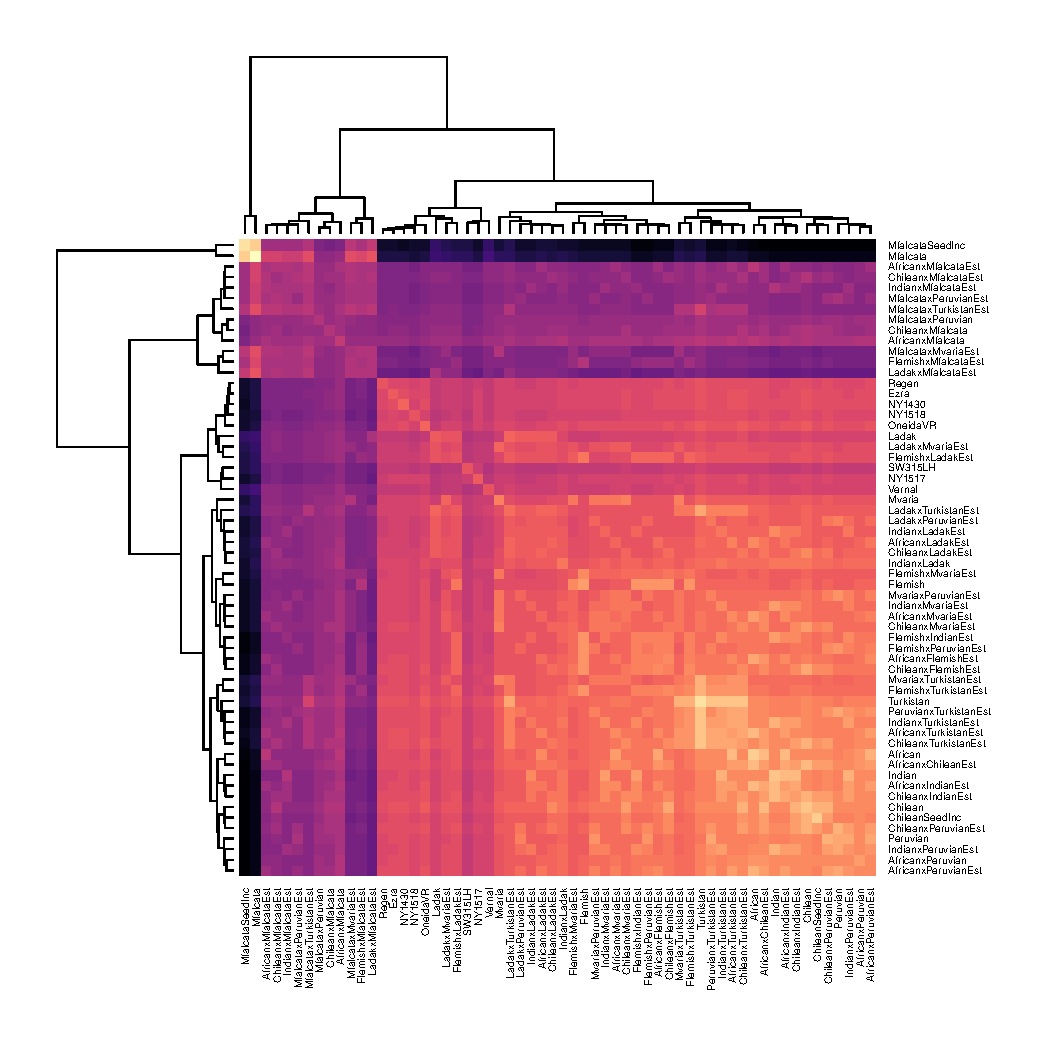
\includegraphics[width = \linewidth, clip, trim = 0cm 0cm 0cm 4cm]{Fig1USAFRIupdate}
\caption{Heat map of pairwise $F_{st}$ values between populations, with rows and columns sorted using hierarchical clustering. Brighter colors indicate higher $F_{st}$ values, and therefore higher additive genetic covariance between populations. Population names ending with ``Est'' have been estimated from their respective parents' allele frequencies.}
\label{heatmap}
\end{figure}


A total of 77,688,674 polymorphic sites were identified in the panel of 22 alfalfa populations. Filtering to keep sites with at least 20, but no more than 125 reads to estimate allele frequencies for each population produced a total of 273,939 sites. These were filtered to obtain global allele frequencies of $0.1 < p < 0.9$ across all populations, resulting in 89,908 sites for estimating genetics relationships across populations. The drastic reduction of sites is primarily due to sampling, where sites were only kept if \emph{every} population had at least 20$\times$ coverage at that site. Because a resequencing approach was used in this study, sites where all populations had sufficient coverage were few, but should be less of a problem in a designed sequence-based marker platform where expected coverage can be increased at little expense if the number of targeted sites is relatively few (say $<$ 100,000 sites). 

% Of the two methods used to estimate genetic relationships, the simple covariance of allele frequencies tended to be more stable for model fitting, suggesting that estimating the gentic covariance based on pairwise $F_{st}$ statistics does not produce a positive definite matrix. This is likely due to the unknown (i.e. because the reference (or basal?)  Fst cannot be estimated due to lack of degrees of freedom, the matrix has a rank < n (likely n-1 or 2)) limitations of. Further investigation is required to determine how this arises. 

% Correlations between expected and empirical allele frequency estimates for the diallel population hybrids was very high, ranging from 0.9 to 0.9, further validating the ability of sequenced based methods to accurately sample alleles and estimate frequency, even in bulk samples with unbalanced numbers of cells per individual, given sufficient individuals are included inthe bulk (i.e. large sample size).

% Genetic relationships were similar to those estimated in the same population lusing AFLPs (Segovia Lerma 2004), with families clustering together (see figure X), especially 


Estimates of hybrid population allele frequencies based on parental population frequencies were highly correlated with those observed in the five hybrid populations from the diallel that were included in the sequencing, ranging from 0.88 to 0.91, and tended to cluster together (Figure \ref{heatmap}). The two cases of biological replicates (`Chilean' and `ChileanSeedInc', and `Mfalcata', `MfalcataSeedInc') were also highly correlated at 0.9 and 0.91 respectively, and subsequently reflected by tight clustering. These high correlations confirm hybrid parentage and the ability to construct hybrid genotypes \emph{in silico}. 

The most genetically distinct population was M. falcata, highlighting its long recognition as a subspecies of \emph{M. sativa}, \emph{M. sativa} subsp. \emph{falcata} \parencite{oakley1917}. Diallel families tended to cluster together, with the least related parent tending to drive the clustering (e.g. families with M. falcata). These results validate the ability of a sequenced-based method to accurately sample alleles and estimate their frequency, even in bulk samples with unequal numbers of cells per individual, given sufficient individuals are included in the bulk.

% , as well as demonstrate the efficacy of the bulk genotyping approach to sample the true  allele frequencies within populations.

% Population level, whole-genome sequencing has been completed for all eight varieties under field evaluation, as well as nine parent populations from the diallel study \parencite{segovia2004}, and five of their diallel hybrids for validation. Bi-allelic variant calling has been performed against the tetraploid alfalfa genome provided by the Noble Research Institute, and we have produced 89,908 sites under strict filtering. Only sites with at least 20$\times$, but no more than 125$\times$, coverage for all populations were kept. Genotypes were further filtered to only include sites with a mean reference allele frequency greater than 0.1 or less than 0.9. We have yet to test the effects of allowing more than 2 alleles or different filtering parameters, but will be carried out at a later date. 

\subsection{Genetic covariance between populations}


% Due to a lack of full rank, the inversion issues 

\subsubsection{Cornell materials}

\begin{table}[t]
\caption{Leave one out genomic prediction accuracy for genetic covariances estimated by pairwise $F_{st}$ or covariance of allele frequencies (covAF) in the Cornell trial in Geneva, NY.}
\label{tab:loo}
\centering
\begin{tabular*}{\hsize}{@{\extracolsep{\fill}}lcrr}
% \begin{tabular}{lrrr}
  % \hline
 Harvest & Year & $F_{st}$ & covAF \\ 
  \hline
  2 & 2019 & 0.27 & 0.43 \\ 
  3 & 2019 & 0.75 & 0.73 \\ 
  1 & 2020 & 0.51 & 0.24 \\ 
  2 & 2020 & 0.94 & 0.97 \\ 
  Sum of 4 harvests & - & 0.90 & 0.79 \\ 
   \hline
\end{tabular*}
\end{table}


The off diagonal elements of the additive genetic covariance calculated as pairwise $F_{st}$ values or as the covariance of allele frequencies were correlated at 0.79 in the Cornell materials. Neither performed uniformly better than the other for genomic prediction of additive forage yield effects effects, but the pairwise $F_{st}$ values tended to perform better for prediction, especially for the sum of the four harvests detailed in this report (Table \ref{tab:loo}). The higher trend in prediction accuracy coupled with the foundation in population genetics theory, resulted in pairwise $F_{st}$'s being used as the estimate of genetic relatedness for the remainder of this report.

\subsubsection{Historic germplasm diallel}

\begin{figure}
% \includegraphics[width = \linewidth]{"\string~/Dropbox/checkoffUpdate2020/Fig2USAFRIupdate"}
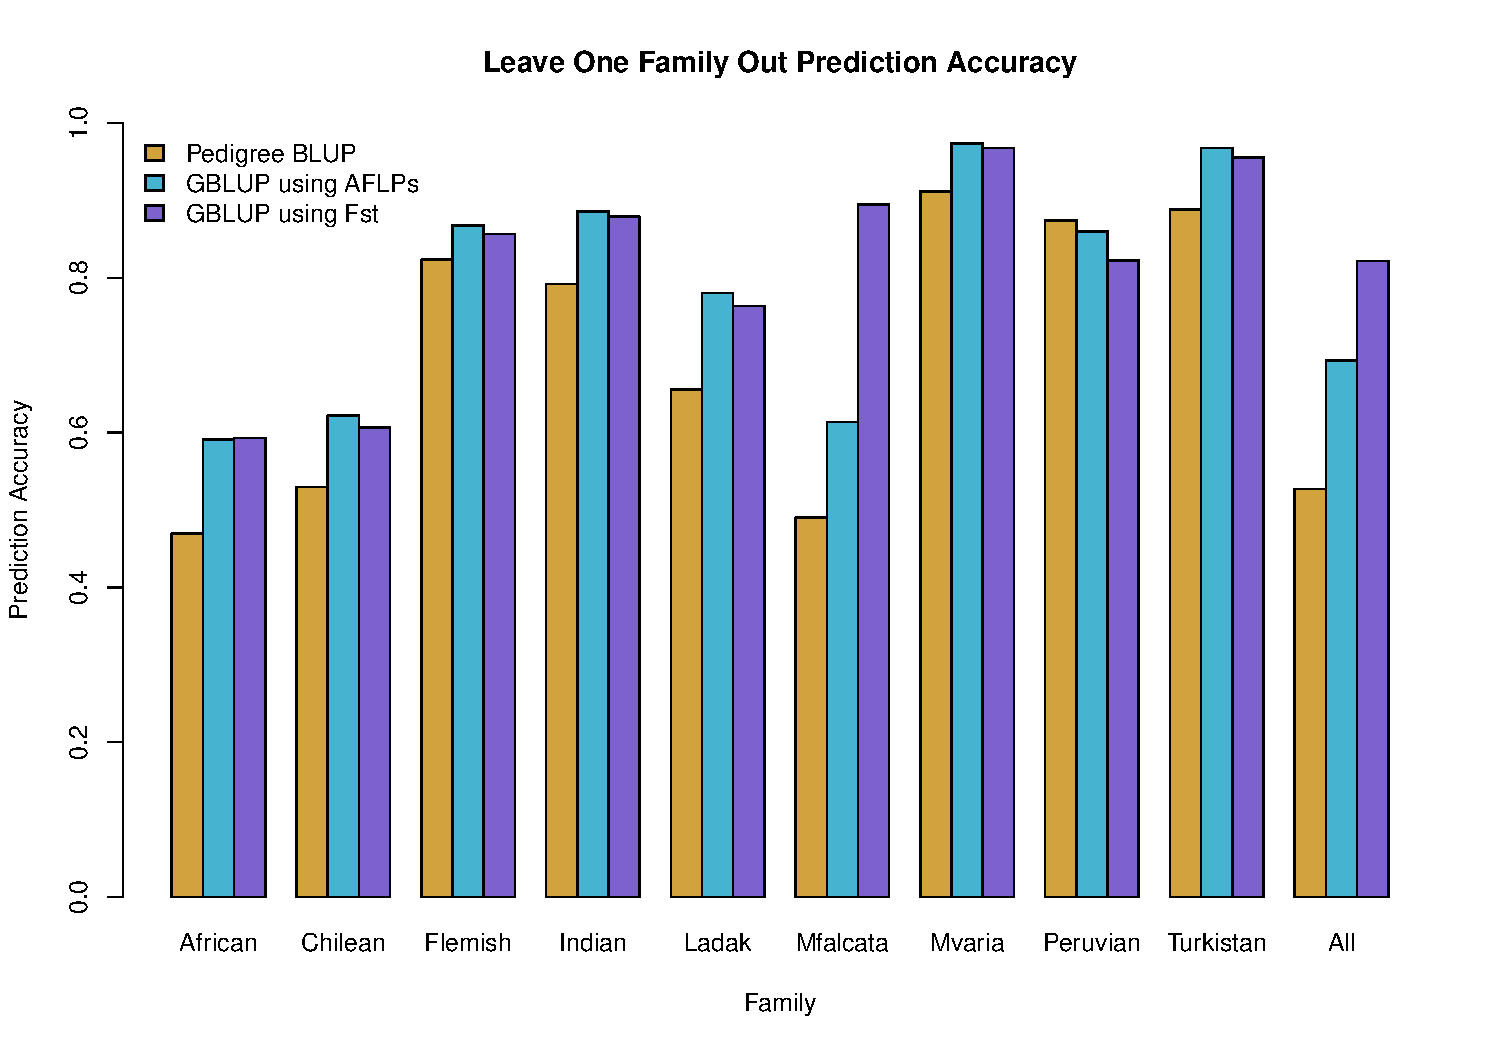
\includegraphics[width = \linewidth]{FstLeaveOneFamOutPredAcc}
\caption{Prediction accuracy using a leave one family out strategy for a diallel population with 9 parental populations, and 36 hybrid populations of alfalfa. For each of the nine parents, all entries with that parent were removed and predicted using the remaining eight families and the additive genetic covariance estimated using pedigrees, dominant markers \parencite[1544 AFLPs;][]{segovia2003}, or $F_{st}$ statistics calculated from variant frequencies determined by whole-genome resequencing.}
\label{diallelpredacc}
\end{figure}

Pairwise $F_{st}$'s \parencite{weir2002} were compared to relationships estimated from AFLP data \parencite[1544 AFLPs;][]{segovia2003}) to compare a sequenced-based marker platform that can estimate allele frequencies with one that can only detect presence or absence (i.e. dominant markers). Genomic predictive ability of yearly dry matter forage yield in the diallel population was used to assess these two marker platform types. The high level of genetic variability and relatedness in the diallel was demonstrated by an unusually high genomic predictability, with leave-one-family-out genomic prediction accuracies ranging from 0.55-0.97 (Figure \ref{diallelpredacc}). $F_{st}$'s showed increased or similar overall predictive ability over pedigree or dominant markers (AFLPs), especially for the most highly unrelated family with the M. falcata parent. This suggests that tracking allele frequencies at many loci better captures relationships between sites and causal loci, rather than simply tracking familial relationships. 

Importantly, this highlights the need of an affordable, medium-density sequence-based marker platform that can estimate allele frequencies. We are currently collaborating with Breeding Insight at Cornell University to include highly polymorphic and informative regions that can distinguish a wide array of North American alfalfa germplasm into a marker panel currently under development.

% Generally, inclusion of marker information increased prediction accuracy compared to a pedigree based prediction model. Inclusion of dominance predictors also increased accuracy for several families, demonstrating that dominance effects are important contributors, and will allow for prediction of hybrid vigor. This data set is atypical in the genetic signal due to the large genetic variability and known recent familial relationships, but we chose this population as a proof of concept because it is small (low cost), and has a high potential to detect differences (high genetic variance). 

% [paragraph about comparison in Fst being better than simple covariance]


\subsection{Phenotypic description}

% \begin{table}[ht]
% \caption{Trait means, heritability and ANOVA p-values for forage yield, crude protein and neutral detergent fiber across 2 harvests in each of 2019 and 2020 for all fifteen entries, or only the eight entries with genotypic information.}
% \centering
% \begin{tabular*}{\hsize}{@{\extracolsep{\fill}}lccrrrrrr}
% % \begin{tabular}{rrrrrr}
%   % \hline
%  trait & year & harvest & \begin{tabular}{c} mean \\ kg ha$^{-1}$ \end{tabular} & iidh2 & iidh28 & covh28 & anovaPval & anovaPval8 \\ 
%   \hline
%   Forage yield & 2019 & 2           & 1.51  & 0.11 & 0.11 & 0.00 & 0.1073 & 0.1751 \\ 
%   Crude Protein & 2019 & 2           & 0.18 & 0.07 & 0.04 & 0.00 & 0.1888 & 0.3219 \\ 
%   ND F & 2019 & 2 & 0.47 & 0.15 & 0.14 & 0.1200 & 0.0478 & 0.1196 \\ 
%   Forage yield & 2019 & 3            & 0.99 & 0.21 & 0.31 & 0.40 & 0.0117 & 0.0110 \\ 
%   Forage yield & 2020 & 1            & 2.65 & 0.40 & 0.24 & 0.24 & $< 0.0001$ & 0.0326 \\ 
%   Forage yield & 2020 & 2            & 1.44 & 0.71 & 0.63 & 0.71 & $< 0.0001$ & $< 0.0001$ \\ 
%   Crude Protein & 2020 & 2           & 0.24 & 0.42 & 0.43 & 0.57 & $< 0.0001$ & 0.0012 \\ 
%   ND F & 2020 & 2 & 0.43 & 0.00 & 0.00 & 0.00 & 0.7521 & 0.7195 \\ 
%    \hline
% \end{tabular*}
% \end{table}

\begin{table}[ht]
\caption{Trait means, heritability and ANOVA p-values for forage yield, crude protein and neutral detergent fiber across 2 harvests in each of 2019 and 2020 for the eight Cornell entries with genotypic information.}
\centering
\begin{tabular*}{\hsize}{@{\extracolsep{\fill}}lccrrrr}
% \begin{tabular*}{rrrrr}
  % \hline
 Trait & Year & Harvest & Harvest Mean & $^\dagger h^2_\text{iid}$ & $^\ddagger h^2_{F_{st}}$ & ANOVA P-value \\ 
  \hline
  Forage yield & 2019 & 2 & 1.51 & 0.11 & 0.41 & 0.1751 \\ 
  Crude Protein & 2019 & 2 & 0.18 & 0.04 & 0.21 & 0.3219 \\ 
  NDF & 2019 & 2 & 0.47 & 0.14 & 0.49 & 0.1196 \\ 
  Forage yield & 2019 & 3 & 0.99 & 0.31 & 0.69 & 0.0110 \\ 
  Forage yield & 2020 & 1 & 2.65 & 0.24 & 0.62 & 0.0326 \\ 
  Forage yield & 2020 & 2 & 1.44 & 0.63 & 0.87 & $<0.0001$ \\ 
  Crude Protein & 2020 & 2 & 0.24 & 0.43 & 0.78 & 0.0012 \\ 
  NDF & 2020 & 2 & 0.43 & 0.00 & 0.00 & 0.7195 \\ 
   \hline
\end{tabular*}
\raggedright
$^\dagger$ Broad Sense heritability estimated by treating entries as independent and identically distributed \\
$^\ddagger h^2_{F_{st}}$ Narrow sense heritability estimated by allowing entries to have a covariance estimated with pairwise $F_{st}$.
\label{anovaTab}
\end{table}

Trait means and heritabilities are shown in Table \ref{anovaTab}. Harvests with higher mean forage yields tended to have lower heritability, suggesting that some stress may allow for better genetic separation of populations. Most traits had significant genetic effects at $P < 0.05$ when analyzed using a simple ANOVA F-test that assumes lines are independent, with the exception of all traits in the second harvest of 2019, and NDF in 2020. Heritabilities increased when genetic relationships as calculated by pairwise $F_{st}$ were used to capture genetic relationships between populations, and therefore share information. 

% [paragraph noting the genetic variability of lack thereof in harvests for end use traits ]

\subsection{Genetic parameters}

Genetic correlations of forage yield between harvests were high (Table \ref{genCorYld}), but low enough to warrant data collection across multiple harvests to get good estimates of total forage output, as is standard practice. Error correlations between adjacent harvests within the same year were quite high, suggesting there are environmental effects within years that have lagging effects. For example, the negative effect of a particularly dry patch may carry over to the next harvest because the ground is still dry. As expected, NDF is highly positively correlated with forage yield, while protein is negatively correlated with both NDF and yield (Tables \ref{genCorQual19} and \ref{genCorQual20}). These trends held true even in the second harvest of 2019, where there was little genetic signal for quality traits. 



\begin{table}[ht]
\caption{Narrow sense heritability (diagonal), and genetic (above diagonal) and residual (below diagonal) correlations of forage yield by harvest.}
\centering
\begin{tabular*}{\hsize}{@{\extracolsep{\fill}}lrrrr}
% \begin{tabular}{lrrrr}
  % \hline
 & Harvest 2, 2019 & Harvest 3, 2019 & Harvest 1, 2020 & Harvest 2, 2020 \\ 
  \hline
Harvest 2, 2019 & 0.11 & 0.63 & 0.85 & 0.71 \\ 
  Harvest 3, 2019 & 0.86 & 0.21 & 0.88 & 0.62 \\ 
  Harvest 1, 2020 & -0.26 & -0.14 & 0.40 & 0.74 \\ 
  Harvest 2, 2020 & -0.06 & 0.05 & 0.35 & 0.71 \\ 
   \hline
\end{tabular*}
\label{genCorYld}
\end{table}


\begin{table}[ht]
\caption{Narrow sense heritability (diagonal), and genetic (above diagonal) and residual (below diagonal) correlations of forage yield (FY) and quality traits, crude protein (CP) and neutral detergent fiber (NDF) for Harvest 2, 2019.}
\centering
\begin{tabular*}{\hsize}{@{\extracolsep{\fill}}lrrr}
% \begin{tabular}{rrrr}
  % \hline
 & FY 2019 & CP 2019 & NDF 2019 \\ 
  \hline
FY 2019 & 0.49 & -0.99 & 0.99 \\ 
  CP 2019 & 0.49 & 0.38 & -0.99 \\ 
  NDF 2019 & 0.25 & -0.30 & 0.49 \\ 
   \hline
\end{tabular*}
\label{genCorQual19}
\end{table}


\begin{table}[ht]
\caption{Narrow sense heritability (diagonal), and genetic (above diagonal) and residual (below diagonal) correlations of forage yield (FY) and quality traits, crude protein (CP) and neutral detergent fiber (NDF) for Harvest 2, 2020.}
\centering
\begin{tabular*}{\hsize}{@{\extracolsep{\fill}}lrrr}
% \begin{tabular}{rrrr}
  % \hline
 & FY 2020 & CP 2020 & NDF 2020 \\ 
  \hline
FY 2020 & 0.88 & -0.98 & 0.91 \\ 
  CP 2020 & -0.30 & 0.78 & -0.84 \\ 
  NDF 2020 & 0.03 & -0.26 & 0.23 \\ 
   \hline
\end{tabular*}
\label{genCorQual20}
\end{table}


\subsection{Genetic relationships between NDVI and forage yield and quality}	


\begin{figure}
% \vspace{-2.3cm}
% \hspace{-1cm}
\centering
 \begin{tikzpicture}

 \begin{scope}[xshift=-4cm, yshift=8cm, scale=0.3]
    \node () at (0,0) {\textbf{Year 2019}};
  \end{scope}

  \begin{scope}[xshift=4cm, yshift=8cm, scale=0.3]
    \node () at (0,0) {\textbf{Year 2020}};
  \end{scope}

%%%%%%%%%%%%%%%%%%
%   \begin{scope}[xshift=-9cm, yshift=9cm, scale=0.3]
%     \node[rotate = 90] () at (0,0) {Harvest 2, 2019};
%   \end{scope}

% \begin{scope}[xshift=-9cm, yshift=3cm, scale=0.3]
%     \node[rotate = 90] () at (0,0) {Harvest 3, 2019};
%   \end{scope}

% \begin{scope}[xshift=-9cm, yshift=-3cm, scale=0.3]
%     \node[rotate = 90] () at (0,0) {Harvest 1, 2020};
%   \end{scope}

% \begin{scope}[xshift=-9cm, yshift=-9cm, scale=0.3]
%     \node[rotate = 90] () at (0,0) {Harvest 2, 2020};
%   \end{scope}

%%%%%%%%%%%

  \begin{scope}[xshift=-4cm, yshift=4cm, scale=1]
    \node () at (0,0) {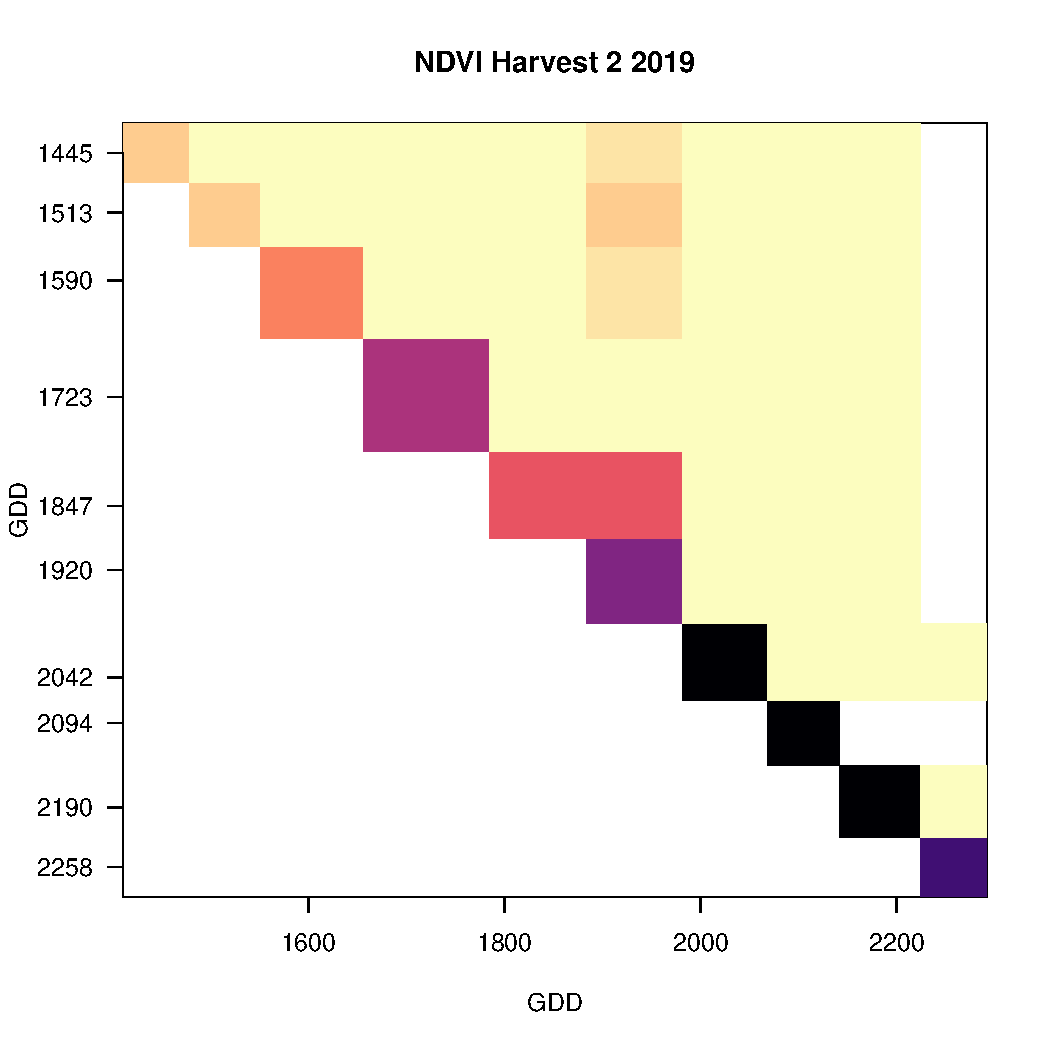
\includegraphics[width = 8cm, page = 1]{heritabilityOfVI}};
  \end{scope}

  \begin{scope}[xshift=4cm, yshift=4cm, scale=1]
    \node () at (0,0) {\includegraphics[width = 8cm, page = 3]{heritabilityOfVI}};
  \end{scope}

  \begin{scope}[xshift=-4cm, yshift=-4cm, scale=1]
    \node () at (0,0) {\includegraphics[width = 8cm, page = 2]{heritabilityOfVI}};
  \end{scope}

  \begin{scope}[xshift=4cm, yshift=-4cm, scale=1]
    \node () at (0,0) {\includegraphics[width = 8cm, page = 4]{heritabilityOfVI}};
  \end{scope}

  \begin{scope}[xshift=-8.5cm, yshift=-6cm, scale=1]
    \node () at (0,0) {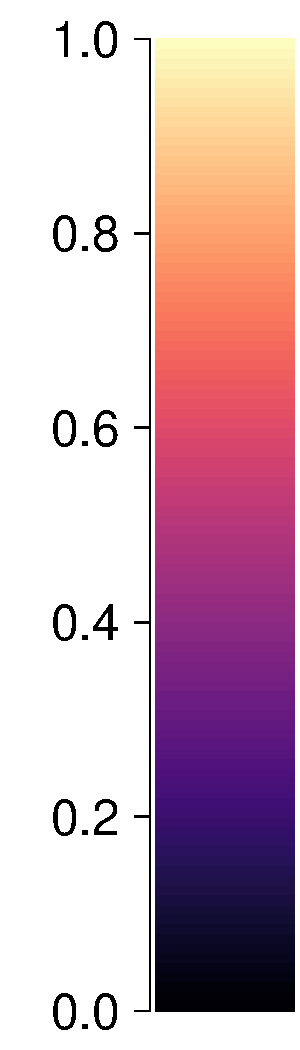
\includegraphics[width = 1cm, page = 1]{legend0to1}};
  \end{scope}

 \end{tikzpicture}
% \vspace{-1cm}
\caption{Heritability (diagonal) of NDVI time points and their genetic correlations (above diagonal) with other time points for four harvests in 2019 and 2020. White blocks indicate that the model failed to converge. Genetic correlations were estimated in  bivariate models for all pairwise combinations of time points.  Many genetic correlation parameters were estimated on the boundary (i.e. very close to 1), and caused model convergence issues.}
\label{genCorVI}
\end{figure}


\begin{figure}
% \vspace{-2.3cm}
% \hspace{-1cm}
\centering
 \begin{tikzpicture}

 \begin{scope}[xshift=-4cm, yshift=8cm, scale=0.3]
    \node () at (0,0) {\textbf{Year 2019}};
  \end{scope}

  \begin{scope}[xshift=4cm, yshift=8cm, scale=0.3]
    \node () at (0,0) {\textbf{Year 2020}};
  \end{scope}

%%%%%%%%%%%%%%%%%%
  \begin{scope}[xshift=-8.5cm, yshift=4cm, scale=0.3]
    \node[rotate = 90] () at (0,0) {Harvest 2};
  \end{scope}

\begin{scope}[xshift=-8.5cm, yshift=-4cm, scale=0.3]
    \node[rotate = 90] () at (0,0) {Harvest 3};
  \end{scope}

  \begin{scope}[xshift=0.5cm, yshift=4cm, scale=0.3]
    \node[rotate = 90] () at (0,0) {Harvest 1};
  \end{scope}

\begin{scope}[xshift=0.5cm, yshift=-4cm, scale=0.3]
    \node[rotate = 90] () at (0,0) {Harvest 2};
  \end{scope}

%%%%%%%%%%%

  \begin{scope}[xshift=-4cm, yshift=4cm, scale=1]
    \node () at (0,0) {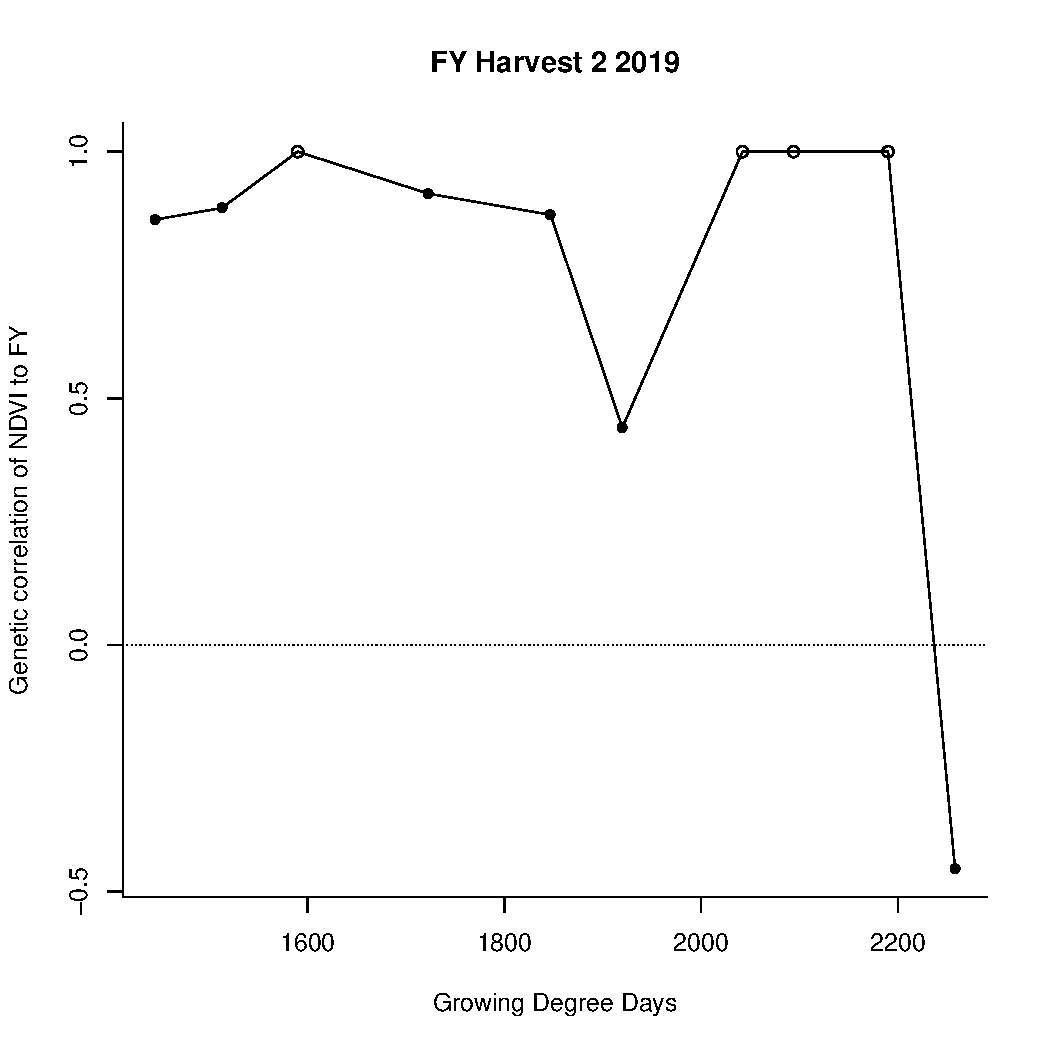
\includegraphics[width = 8cm, page = 1]{corByGDD}};
  \end{scope}

  \begin{scope}[xshift=5cm, yshift=4cm, scale=1]
    \node () at (0,0) {\includegraphics[width = 8cm, page = 4]{corByGDD}};
  \end{scope}

  \begin{scope}[xshift=-4cm, yshift=-4cm, scale=1]
    \node () at (0,0) {\includegraphics[width = 8cm, page = 5]{corByGDD}};
  \end{scope}

  \begin{scope}[xshift=5cm, yshift=-4cm, scale=1]
    \node () at (0,0) {\includegraphics[width = 8cm, page = 6]{corByGDD}};
  \end{scope}

 \end{tikzpicture}
% \vspace{-1cm}
\caption{Genetic correlations of NDVI time points with forage yield four harvests in 2019 and 2020. Open circles indicate genetic correlation parameter that were estimated on the boundary (i.e. very close to 1). Genetic correlations were estimated in in bivariate models for all pairwise combinations of time points and the end-use trait.}
\label{genCorVItraits}
\end{figure}


Bivariate models were used to estimate genetic correlations for all pairwise combinations of time points and forage yield. NDVI time points tended to have very high genetic correlations to adjacent time points (Figure \ref{genCorVItraits}) as well as to forage yield (Figure \ref{genCorVI}), so much that it created a problem with model fitting and convergence. Many genetic correlation coefficients were estimated on the boundary (i.e. very close to 1), and some models failed to converge at all. While a larger data set may resolve such issues, it seems likely that there is a high degree of genetic relationship between vegetative indices like NDVI and forage yield, indicating that they should make good predictors of performance without having to observe the end-use phenotype. 

% latex table generated in R 3.5.0 by xtable 1.8-4 package
% Sat Aug 29 14:50:42 2020


% \subsection{Prediction of unobserved harvests and replications}

\subsection{Using Vegetative indices to predict unobserved phenotypes}

Informative VIs used for prediction were determined by heritability and genetic correlations, and were at Julian days 194 and 223 (GDDs 1723 and 2590) for the second and third harvests in 2019, and Julian days 125 and 183 (GDDs 198 and 1420) for the first and second harvest in 2020. 

Using vegetative indices to predict forage yield without phenotypic data yielded mixed results. Generally, prediction of completely unobserved harvests was improved by using genetic relationships, and was often improved further by observing an informative VI, although this depended upon the harvest that was being predicted and which harvests were available to train the model on. The use of the first PC of the matrix of NDVI time points was often the best model, but also resulted in negative accuracy when the third harvest of 2019 and the second harvest of 2020 were used to train the model. The results warrant caution for the use of NDVI as a surrogate for forage yield. Further investigation with a larger study is needed to determine the efficacy of using vegetative indices to replace a plot harvester. Inclusion of genetic relationships did however, uniformly improve prediction of unobserved harvests over using simple means from observed ones. 

Inclusion of NDVI did not improve prediction of genetic values when some replicates were missing \ref{predRepsMean}. Instead allowing for genetic relatedness of populations was the best strategy to predict yield with reduced replication. Adding the extra phenotype appears to add some environmental error to the estimate of genetic merit for forage yield under reduced replications. This highlights the need to use genetic relationships when estimating the genetic merit of new breeding materials, as well as providing a opportunity to reduce replication and increase the number of entries in the trial. An increase in the number of potential new populations will increase selection intensity and the likelihood of identifying superior populations for future release as varieties.

% - predicting harvests with vegetative indices

% - predicting values without harvesting all reps. 
% 	* genetic relationships allow for reduced phenotyping
% 	* unclear if veg indices 

% latex table generated in R 3.5.0 by xtable 1.8-4 package
% Sun Aug 30 19:50:27 2020
\begin{table}[ht]
\caption{\nicholas{\textbf{REMOVE????}} Prediction accuracy of unobserved harvests for forage yield. Either the first principal component of the matrix of NDVI time points (PC), a single informative NDVI time point (VI), or no high throughput phenotype was observed (K and iid) in unobserved harvests. When no high throughput phenotype was used, either populations were allowed to have genetic relationships calculated from pairwise $F_{st}$'s' (K) or were considered independent (iid). For the iid method, simple means of observed plots were used to predict the genetic merit of each population.}
\centering
\begin{tabular*}{\hsize}{@{\extracolsep{\fill}}llrrrr}
% \begin{tabular}{llrrrr}
  \hline
 Unobserved & Observed & VI & PC & K & iid \\ 
  \hline
  FY1\_20 & FY2\_19 FY3\_19 & 0.55 & 0.74 & 0.53 & 0.49 \\ 
  FY2\_20 & FY2\_19 FY3\_19 & 0.90 & 0.94 & 0.76 & 0.71 \\ 
  FY3\_19 & FY2\_19 FY1\_20 & 0.68 & 0.73 & 0.86 & 0.81 \\ 
  FY2\_20 & FY2\_19 FY1\_20 & 0.90 & 0.94 & 0.82 & 0.74 \\ 
  FY3\_19 & FY2\_19 FY2\_20 & 0.68 & 0.73 & 0.93 & 0.94 \\ 
  FY1\_20 & FY2\_19 FY2\_20 & 0.55 & 0.74 & 0.64 & 0.61 \\ 
  FY2\_19 & FY3\_19 FY1\_20 & 0.81 & 0.71 & 0.68 & 0.68 \\ 
  FY2\_20 & FY3\_19 FY1\_20 & 0.90 & 0.94 & 0.88 & 0.84 \\ 
  FY2\_19 & FY3\_19 FY2\_20 & 0.82 & -0.71 & 0.72 & 0.72 \\ 
  FY1\_20 & FY3\_19 FY2\_20 & 0.55 & -0.74 & 0.65 & 0.64 \\ 
  FY2\_19 & FY1\_20 FY2\_20 & 0.82 & 0.71 & 0.55 & 0.54 \\ 
  FY3\_19 & FY1\_20 FY2\_20 & 0.68 & 0.73 & 0.76 & 0.73 \\ 
  FY2\_20 & FY2\_19 FY3\_19 FY1\_20 & 0.90 & 0.94 & 0.84 & 0.80 \\ 
  FY1\_20 & FY2\_19 FY3\_19 FY2\_20 & 0.55 & 0.74 & 0.62 & 0.60 \\ 
  FY3\_19 & FY2\_19 FY1\_20 FY2\_20 & 0.68 & 0.73 & 0.88 & 0.87 \\ 
  FY2\_19 & FY3\_19 FY1\_20 FY2\_20 & 0.81 & 0.71 & 0.66 & 0.67 \\ 
   \hline
\end{tabular*}
\end{table}

\begin{table}[ht]
\caption{\nicholas{\textbf{Need to either keep means or individual accuracies (above table)..}} Mean prediction accuracy of unobserved harvests using either 2 or 3 harvest for prediction}
\centering
\begin{tabular*}{\hsize}{@{\extracolsep{\fill}}lrrrr}
% \begin{tabular}{rrrrrr}
  \hline
 ObsHarv & VI & PC & K & iid \\ 
  \hline
  2 & 0.74 & 0.54 & 0.73 & 0.70 \\ 
  3 & 0.74 & 0.78 & 0.75 & 0.73 \\ 
   \hline
\end{tabular*}
\end{table}

% \begin{table}[ht]
% \caption{\nicholas{\textbf{REMOVE????}} Prediction accuracy of unobserved harvests}
% \centering
% \begin{tabular}{rrrrr}
%   \hline
%  & VI & PC & K & iid \\ 
%   \hline
%   yld1\_20\_yld2\_201 & 0.55 & 0.74 & 0.53 & 0.49 \\ 
%   yld1\_20\_yld2\_202 & 0.90 & 0.94 & 0.76 & 0.71 \\ 
%   yld3\_19\_yld2\_201 & 0.68 & 0.73 & 0.86 & 0.81 \\ 
%   yld3\_19\_yld2\_202 & 0.90 & 0.94 & 0.82 & 0.74 \\ 
%   yld3\_19\_yld1\_201 & 0.68 & 0.73 & 0.93 & 0.94 \\ 
%   yld3\_19\_yld1\_202 & 0.55 & 0.74 & 0.64 & 0.61 \\ 
%   yld2\_19\_yld2\_201 & 0.81 & 0.71 & 0.68 & 0.68 \\ 
%   yld2\_19\_yld2\_202 & 0.90 & 0.94 & 0.88 & 0.84 \\ 
%   yld2\_19\_yld1\_201 & 0.82 & -0.71 & 0.72 & 0.72 \\ 
%   yld2\_19\_yld1\_202 & 0.55 & -0.74 & 0.65 & 0.64 \\ 
%   yld2\_19\_yld3\_191 & 0.82 & 0.71 & 0.55 & 0.54 \\ 
%   yld2\_19\_yld3\_192 & 0.68 & 0.73 & 0.76 & 0.73 \\ 
%   yld2\_20 & 0.90 & 0.94 & 0.84 & 0.80 \\ 
%   yld1\_20 & 0.55 & 0.74 & 0.62 & 0.60 \\ 
%   yld3\_19 & 0.68 & 0.73 & 0.88 & 0.87 \\ 
%   yld2\_19 & 0.81 & 0.71 & 0.66 & 0.67 \\ 
%    \hline
% \end{tabular}
% \label{predHarv}
% \end{table}


\begin{table}[ht]
\caption{Mean accuracy of genetic values when 1 to 4 replications of forage biomass data are set to missing. Either the first principal component of the matrix of NDVI time points (PC), a single informative NDVI time point (VI), or no high throughput phenotype was observed (K and iid) for up to 4 reps for each harvest. When no high throughput phenotype was used, either populations were allowed to have genetic relationships calculated from pairwise $F_{st}$'s' (K) or were considered independent (iid). For the iid method, simple means of observed plots were used to predict the genetic merit of each population.}

\centering
\begin{tabular*}{\hsize}{@{\extracolsep{\fill}}lrrrr}
% \begin{tabular}{rrrrr}
  \hline
 \# observed reps & PC & VI & K & iid \\ 
  \hline
  4 & 0.87 & 0.89 & 0.96 & 0.96 \\ 
  3 & 0.82 & 0.82 & 0.92 & 0.91 \\ 
  2 & 0.81 & 0.77 & 0.85 & 0.82 \\ 
  1 & 0.69 & 0.62 & 0.71 & 0.65 \\ 
   \hline
\end{tabular*}
\label{predRepsMean}
\end{table}

% latex table generated in R 3.5.0 by xtable 1.8-4 package
% Sun Aug 30 08:32:15 2020
% \begin{table}[h]
% \caption{\nicholas{REMOVE!} Mean accuracy of genetic values within harvest when 1 to 4 replications of forage biomass data are set to missing. }
% \centering
% \begin{tabular}{rlrrrrr}
%   \hline
%  & pred & hidden reps & withNDVI & NDVIfixed & noNDVI & iid \\ 
%   \hline
%   FY2\_19 & PC &   1 & 0.66 & 0.61 & 0.92 & 0.94 \\ 
%   FY3\_19 & PC &   1 & 0.96 & 0.95 & 0.97 & 0.97 \\ 
%   FY1\_20 & PC &   1 & 0.89 & 0.94 & 0.95 & 0.96 \\ 
%   FY2\_20 & PC &   1 & 0.99 & 0.86 & 0.99 & 0.99 \\ 
%   FY2\_19.1 & PC &   2 & 0.51 & 0.51 & 0.87 & 0.85 \\ 
%   FY3\_19.1 & PC &   2 & 0.92 & 0.89 & 0.93 & 0.92 \\ 
%   FY1\_20.1 & PC &   2 & 0.86 & 0.89 & 0.90 & 0.90 \\ 
%   FY2\_20.1 & PC &   2 & 0.98 & 0.81 & 0.97 & 0.97 \\ 
%   FY2\_19.2 & PC &   3 & 0.58 & 0.41 & 0.75 & 0.72 \\ 
%   FY3\_19.2 & PC &   3 & 0.86 & 0.81 & 0.88 & 0.84 \\ 
%   FY1\_20.2 & PC &   3 & 0.84 & 0.79 & 0.82 & 0.80 \\ 
%   FY2\_20.2 & PC &   3 & 0.97 & 0.74 & 0.95 & 0.94 \\ 
%   FY2\_19.3 & PC &   4 & 0.28 & 0.24 & 0.53 & 0.49 \\ 
%   FY3\_19.3 & PC &   4 & 0.79 & 0.62 & 0.79 & 0.76 \\ 
%   FY1\_20.3 & PC &   4 & 0.75 & 0.68 & 0.73 & 0.66 \\ 
%   FY2\_20.3 & PC &   4 & 0.95 & 0.64 & 0.80 & 0.80 \\ 
%   FY2\_191 & VI &   1 & 0.83 & 0.34 & 0.92 & 0.94 \\ 
%   FY3\_191 & VI &   1 & 0.90 & 0.85 & 0.97 & 0.97 \\ 
%   FY1\_201 & VI &   1 & 0.84 & 0.92 & 0.95 & 0.96 \\ 
%   FY2\_201 & VI &   1 & 0.99 & 0.77 & 0.99 & 0.99 \\ 
%   FY2\_19.11 & VI &   2 & 0.72 & 0.34 & 0.86 & 0.84 \\ 
%   FY3\_19.11 & VI &   2 & 0.86 & 0.80 & 0.93 & 0.92 \\ 
%   FY1\_20.11 & VI &   2 & 0.71 & 0.83 & 0.90 & 0.90 \\ 
%   FY2\_20.11 & VI &   2 & 0.98 & 0.73 & 0.97 & 0.97 \\ 
%   FY2\_19.21 & VI &   3 & 0.67 & 0.28 & 0.75 & 0.71 \\ 
%   FY3\_19.21 & VI &   3 & 0.82 & 0.73 & 0.88 & 0.84 \\ 
%   FY1\_20.21 & VI &   3 & 0.61 & 0.66 & 0.82 & 0.80 \\ 
%   FY2\_20.21 & VI &   3 & 0.96 & 0.69 & 0.95 & 0.94 \\ 
%   FY2\_19.31 & VI &   4 & 0.60 & 0.26 & 0.53 & 0.49 \\ 
%   FY3\_19.31 & VI &   4 & 0.70 & 0.61 & 0.72 & 0.58 \\ 
%   FY1\_20.31 & VI &   4 & 0.26 & 0.43 & 0.73 & 0.66 \\ 
%   FY2\_20.31 & VI &   4 & 0.92 & 0.52 & 0.86 & 0.86 \\ 
%    \hline
% \end{tabular}
% \label{predReps}
% \end{table}


% [two paragraphs about how VIs do increase prediction, but most gain comes from including genetic covariance!]


% Sample mix up: The 

% 2019 forage quality samples appear to have an issue with the data that is most likely a mix up of the samples with their respective plot  identifiers. Neither CP or NDF had significant genotype effects (pvals?) in 2019, while both 2020 quality measurements were significant at p =  , respectively. The clear patterns seen in the 2020 forage quality data suggest that the 2019 data was somehow corrupted. It is currently unlcear where the mistake was made. 


% 	All sequences will be made publicly available before publication. 

% - descriptive
% 	- total of 77,688,674 polymorphic sites
% 	- filtered by --minCnt 20 --maxCnt 125 --minMean 20 --maxMean 75 --minTot 0 --maxTot 10000
% 		. 273,939 sites
% 	- further filtering to get allele frequencies 

% 	* number of sites before / after filtering

% - heatmaps of relationship matrices
% 	* relationships within
% 	* families tend to cluster as expected

% - crossvalidation in diallel
% 	* 

% - crossvalidation in geneva trial 
% 	* CV accuracy of leave one out approach. 





\subsection{Genotype specific growth curves}

\begin{table}[h]
\caption{Genetic correlations of Legendre polynomial parameters, L0, L1, L2, and L3 with forage yield (FY) in all four harvests, and NDF for harvest 2, 2019, and CP for harvest 2 2020. NDF in 2020 and CP in 2019 were not included as they had little to no genetic variation.}
\noindent%
\begin{minipage}[h]{.45\textwidth}
\centering

\textbf{\underline{Year 2019}}

\medskip

Forage Yield Harvest 2

\medskip

\begin{tabular}{rrrrrr}
  % \hline
 & L0 & L1 & L2 & L3 & FY \\ 
  \hline
  L0 &  & -0.99 & 0.88 & 0.28 & 0.76 \\ 
  L1 & &  & -0.87 & -0.32 & -0.77 \\ 
  L2 & & &  & -0.10 & 0.42 \\ 
  L3 & & & &  & 0.78 \\ 
   \hline
\end{tabular}

\bigskip
\bigskip

CP Harvest 2

\medskip

\begin{tabular}{rrrrrr}
  % \hline
 & L0 & L1 & L2 & L3 & CP \\ 
  \hline
  L0 &  & -0.89 & 0.98 & 0.16 & -0.76 \\ 
  L1 & & & -0.95 & -0.56 & 0.70 \\ 
  L2 & & & & 0.31 & -0.75 \\ 
  L3 & & & & & -0.18 \\ 
   \hline
\end{tabular}
\bigskip
\bigskip

NDF Harvest 2

\medskip

\begin{tabular}{rrrrrr}
  % \hline
 & L0 & L1 & L2 & L3 & NDF \\ 
  \hline
  L0 & & -0.89 & 0.98 & 0.17 & 0.92 \\ 
  L1 & & & -0.95 & -0.57 & -0.93 \\ 
  L2 & & & & 0.31 & 0.94 \\ 
  L3 & & & & & 0.38 \\ 
   \hline
\end{tabular}

\bigskip
\bigskip

Forage Yield Harvest 3

\medskip

\begin{tabular}{rrrrrr}
  % \hline
 & L0 & L1 & L2 & L3 & FY \\ 
  \hline
  L0 &  & 0.04 & -0.91 & 0.12 & 0.81 \\ 
  L1 & &  & -0.04 & -0.98 & -0.15 \\ 
  L2 & & &  & -0.11 & -0.95 \\ 
  L3 & & & &  & 0.28 \\ 
   \hline
\end{tabular}
\end{minipage}%
\begin{minipage}[h]{.05\textwidth}
\
\end{minipage}%
\begin{minipage}[h]{.45\textwidth}
\centering

\textbf{\underline{Year 2020}}

\medskip

Forage Yield Harvest 1

\medskip

\begin{tabular}{rrrrrr}
  % \hline
 & L0 & L1 & L2 & L3 & FY \\ 
  \hline
  L0 &   & 0.12 & -0.09 & -0.65 & 0.80 \\ 
  L1 & &   & -0.81 & -0.69 & 0.18 \\ 
  L2 & & &   & 0.62 & 0.17 \\ 
  L3 & & & &   & -0.49 \\ 
   \hline
\end{tabular}

\bigskip
\bigskip

Forage Yield Harvest 2

\medskip

\begin{tabular}{rrrrrr}
  % \hline
 & L0 & L1 & L2 & L3 & FY \\ 
  \hline
  L0 &   & 0.54 & -0.99 & 0.72 & 0.95 \\ 
  L1 & &   & -0.55 & -0.09 & 0.36 \\ 
  L2 & & &   & -0.66 & -0.91 \\ 
  L3 & & & &   & 0.87 \\ 
   \hline
\end{tabular}

\bigskip
\bigskip

CP Harvest 2

\medskip

\begin{tabular}{rrrrrr}
  % \hline
 & L0 & L1 & L2 & L3 & CP \\ 
  \hline
L0 &  & 0.30 & -0.99 & 0.68 & -0.96 \\ 
  L1 & & & -0.19 & -0.47 & -0.22 \\ 
  L2 & & & & -0.74 & 0.94 \\ 
  L3 & & & & & -0.73 \\ 
   \hline
\end{tabular}
\bigskip
\bigskip

NDF Harvest 2

\medskip
\begin{tabular}{rrrrrr}
  \hline
 & L0 & L1 & L2 & L3 & NDF \\ 
  \hline
  L0 & & 0.31 & -0.99 & 0.69 & 0.83 \\ 
  L1 & & & -0.19 & -0.46 & 0.76 \\ 
  L2 & & & & -0.76 & -0.76 \\ 
  L3 & & & & & 0.21 \\ 
   \hline
\end{tabular}

\end{minipage}% <---------------- Note the use of "%"
\end{table}


\begin{figure}
\vspace{-2.3cm}
\hspace{-1cm}
 \begin{tikzpicture}

 \begin{scope}[xshift=-6cm, yshift=12cm, scale=0.3]
    \node () at (0,0) {\textbf{Growth curve deviations}};
  \end{scope}

\begin{scope}[xshift=0cm, yshift=12cm, scale=0.3]
    \node () at (0,0) {\textbf{Growth curves}};
  \end{scope}

\begin{scope}[xshift=6cm, yshift=12.2cm, scale=0.3]
    \node () at (0,0) {\begin{tabular}{c} \textbf{Area under the} \\ \textbf{growth curve (AUGC)} \end{tabular}};
  \end{scope}
%%%%%%%%%%%%%%%%%%
  \begin{scope}[xshift=-9cm, yshift=9cm, scale=0.3]
    \node[rotate = 90] () at (0,0) {Harvest 2, 2019};
  \end{scope}

\begin{scope}[xshift=-9cm, yshift=3cm, scale=0.3]
    \node[rotate = 90] () at (0,0) {Harvest 3, 2019};
  \end{scope}

\begin{scope}[xshift=-9cm, yshift=-3cm, scale=0.3]
    \node[rotate = 90] () at (0,0) {Harvest 1, 2020};
  \end{scope}

\begin{scope}[xshift=-9cm, yshift=-9cm, scale=0.3]
    \node[rotate = 90] () at (0,0) {Harvest 2, 2020};
  \end{scope}

%%%%%%%%%%%

  \begin{scope}[xshift=-6cm, yshift=9cm, scale=0.3]
    \node () at (0,0) {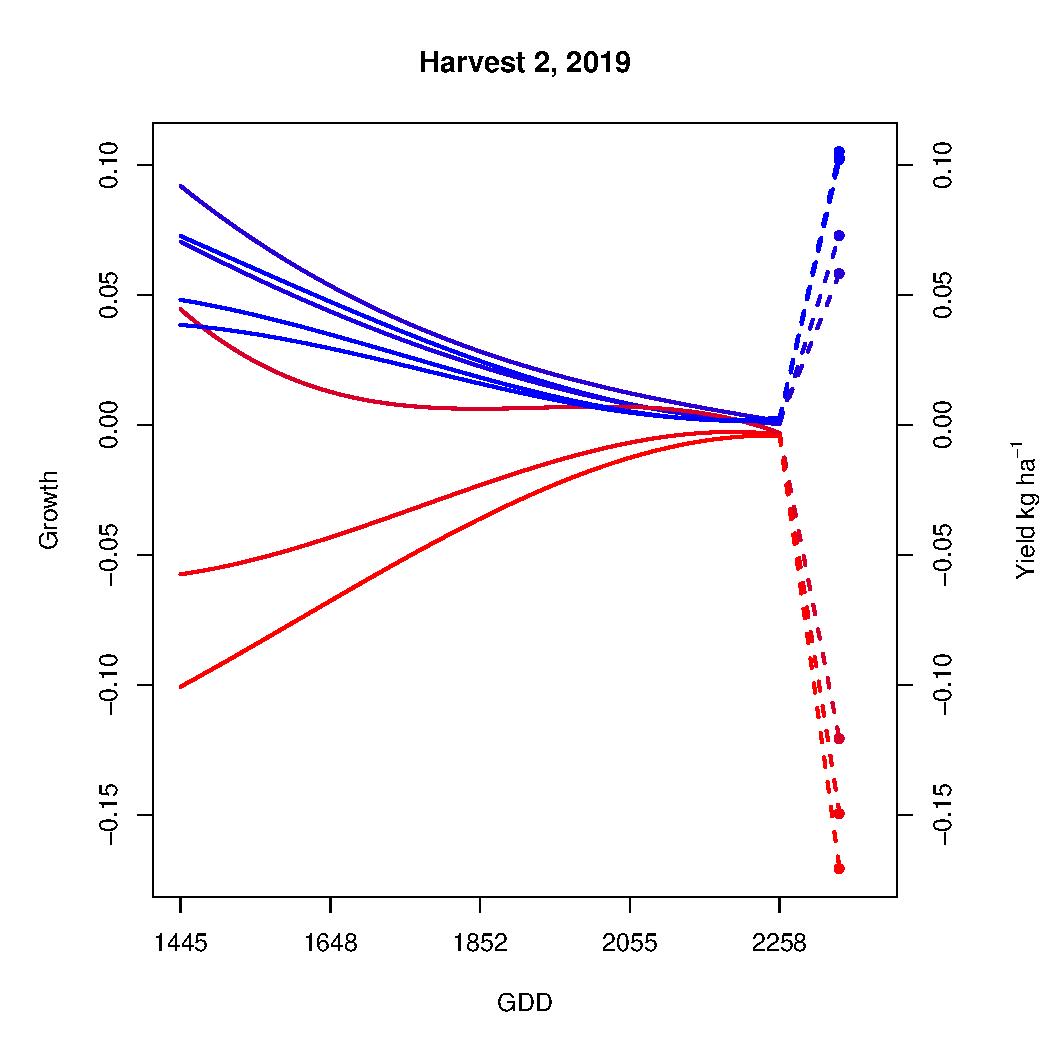
\includegraphics[width = 6cm]{growthCurveDeviations_ndvi_yld_h2_2019_geno8}};
  \end{scope}

  \begin{scope}[xshift=0cm, yshift=9cm, scale=0.3]
    \node () at (0,0) {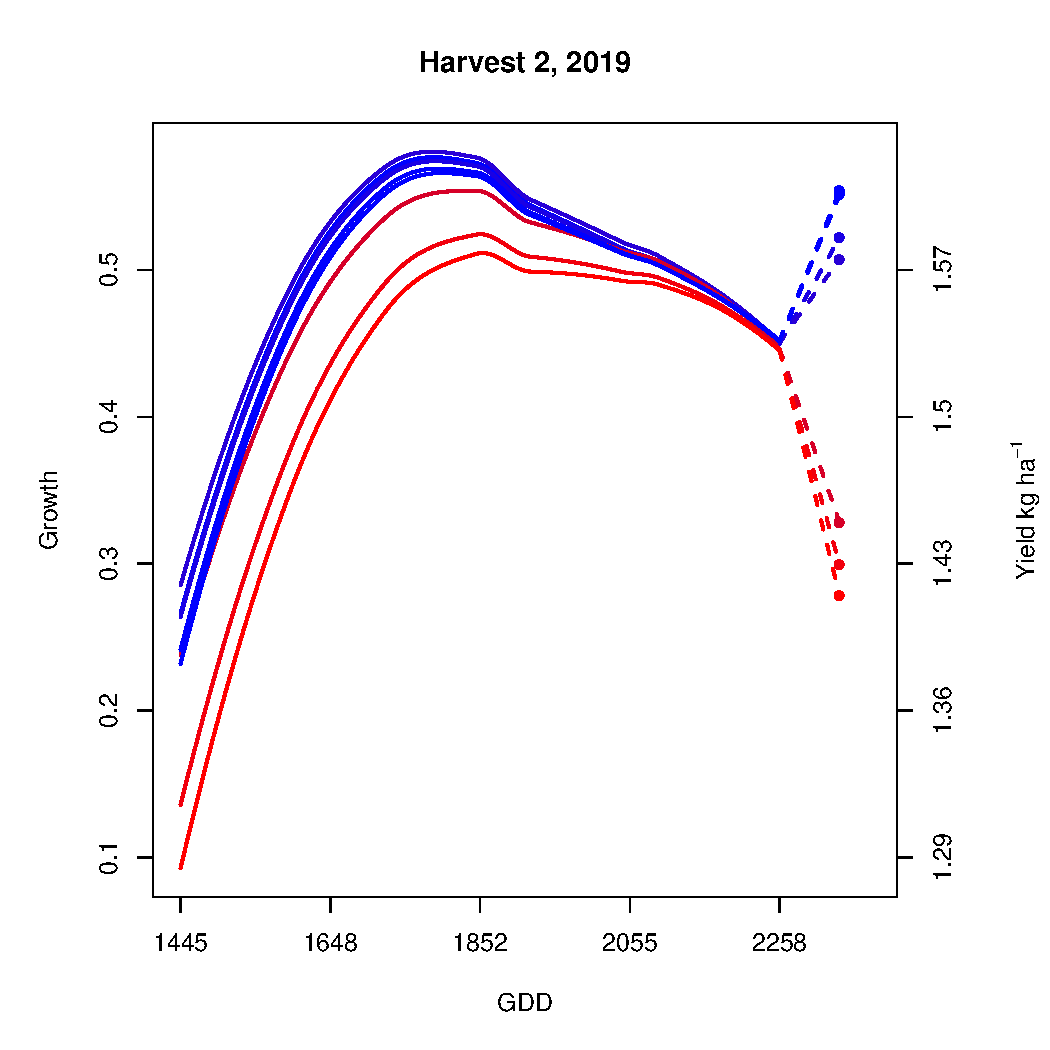
\includegraphics[width = 6cm]{growthCurvesWithMeanCurve_ndvi_yld_h2_2019_geno8}};
  \end{scope}

  \begin{scope}[xshift=6cm, yshift=9cm, scale=0.3]
    \node () at (0,0) {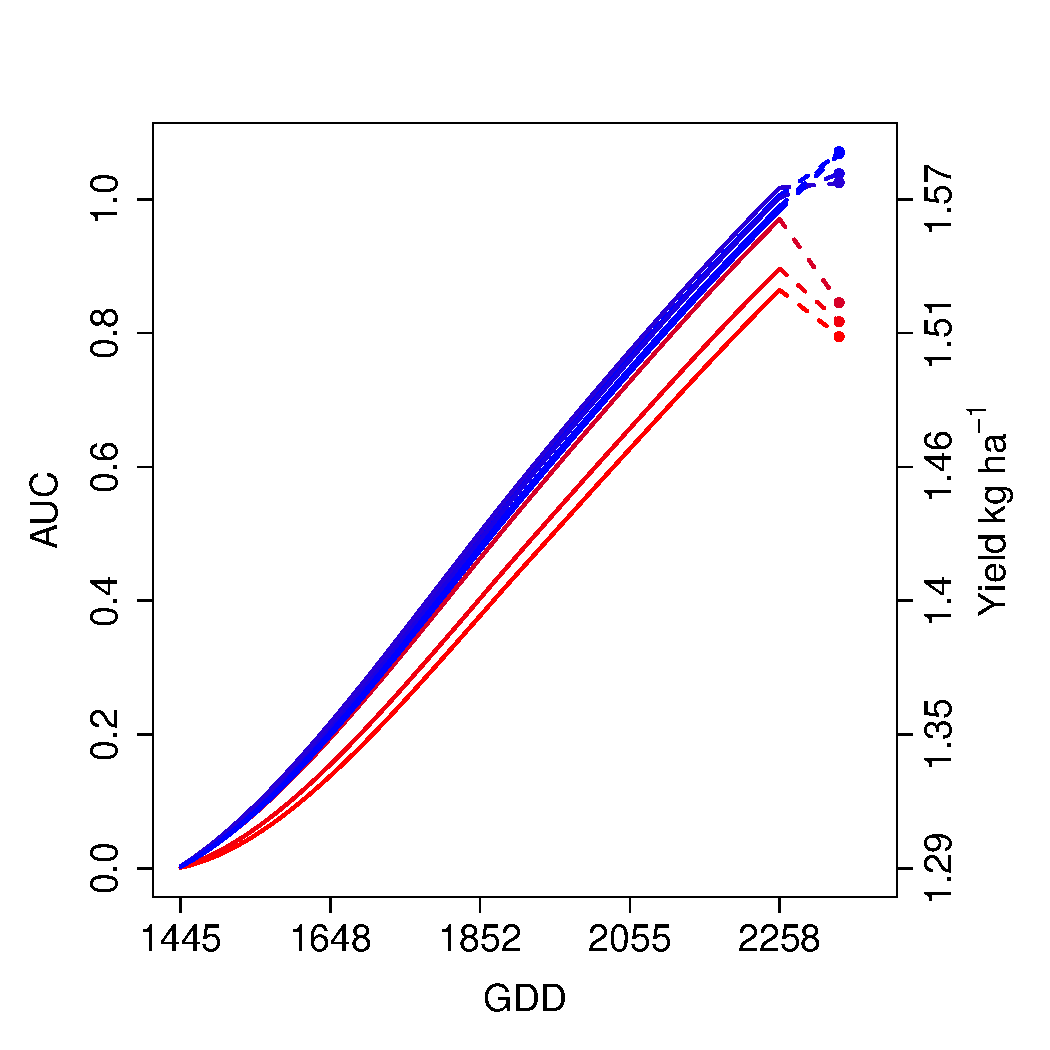
\includegraphics[width = 6cm]{AUC_ndvi_yld_h2_2019_geno8}};
  \end{scope}

  \begin{scope}[xshift=-6cm, yshift=3cm, scale=0.3]
    \node () at (0,0) {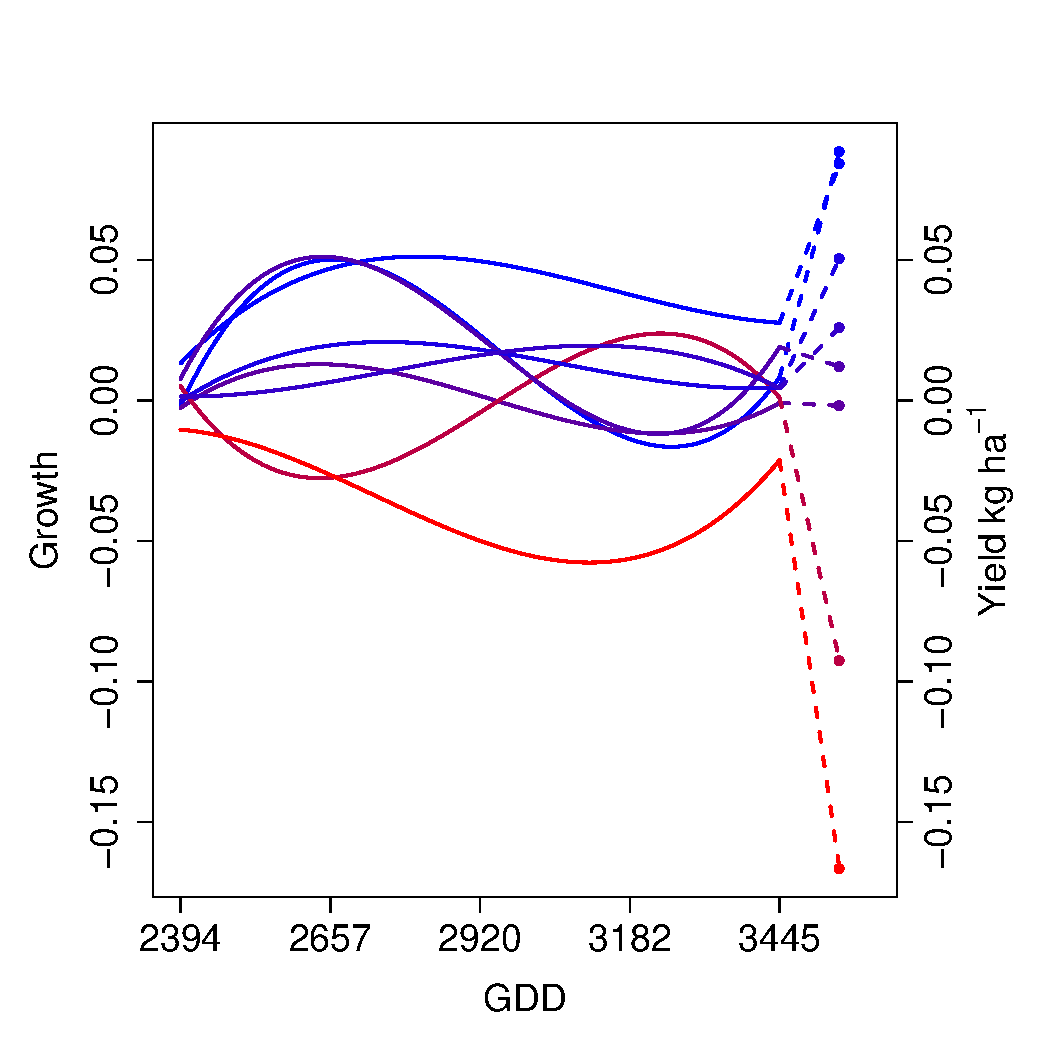
\includegraphics[width = 6cm]{growthCurveDeviations_ndvi_yld_h3_2019_geno8}};
  \end{scope}

  \begin{scope}[xshift=0cm, yshift=3cm, scale=0.3]
    \node () at (0,0) {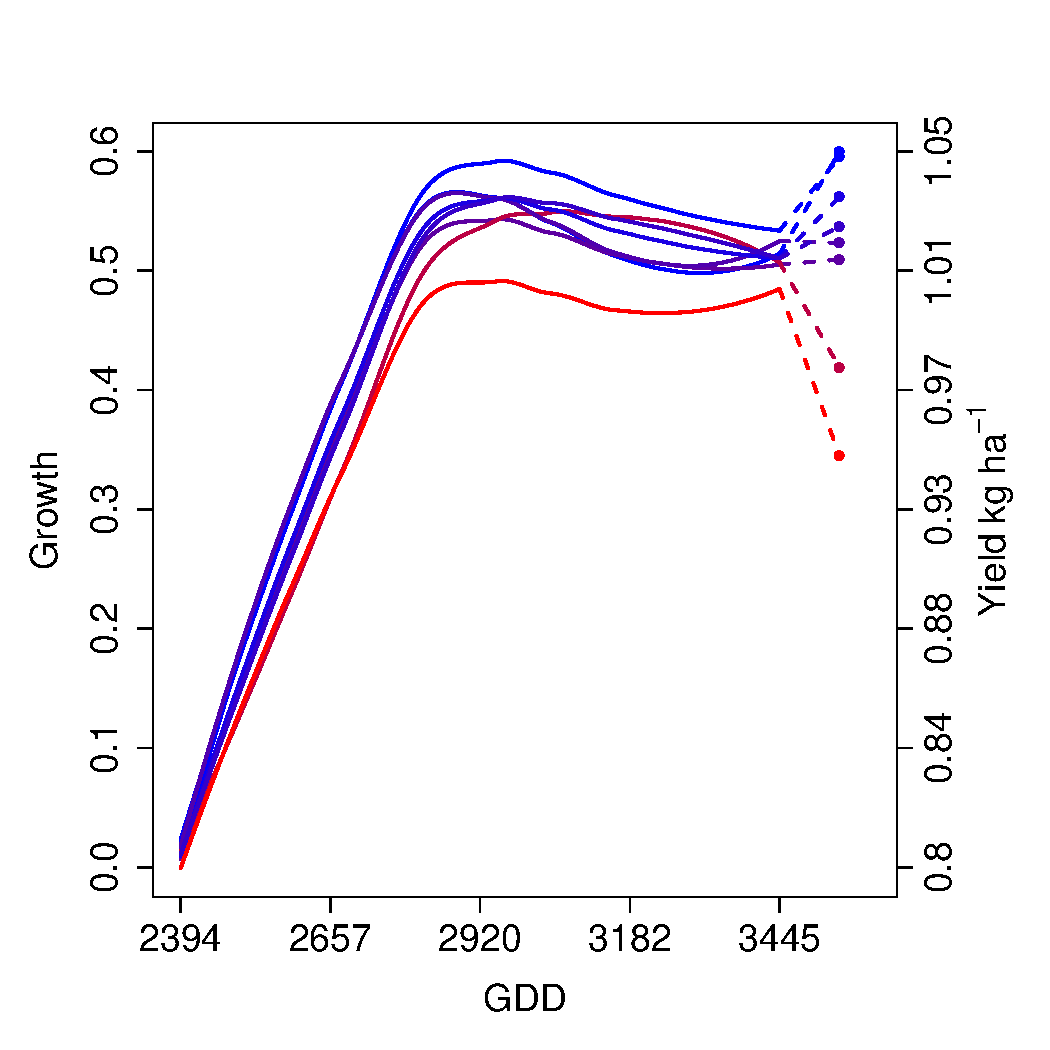
\includegraphics[width = 6cm]{growthCurvesWithMeanCurve_ndvi_yld_h3_2019_geno8}};
  \end{scope}

  \begin{scope}[xshift=6cm, yshift=3cm, scale=0.3]
    \node () at (0,0) {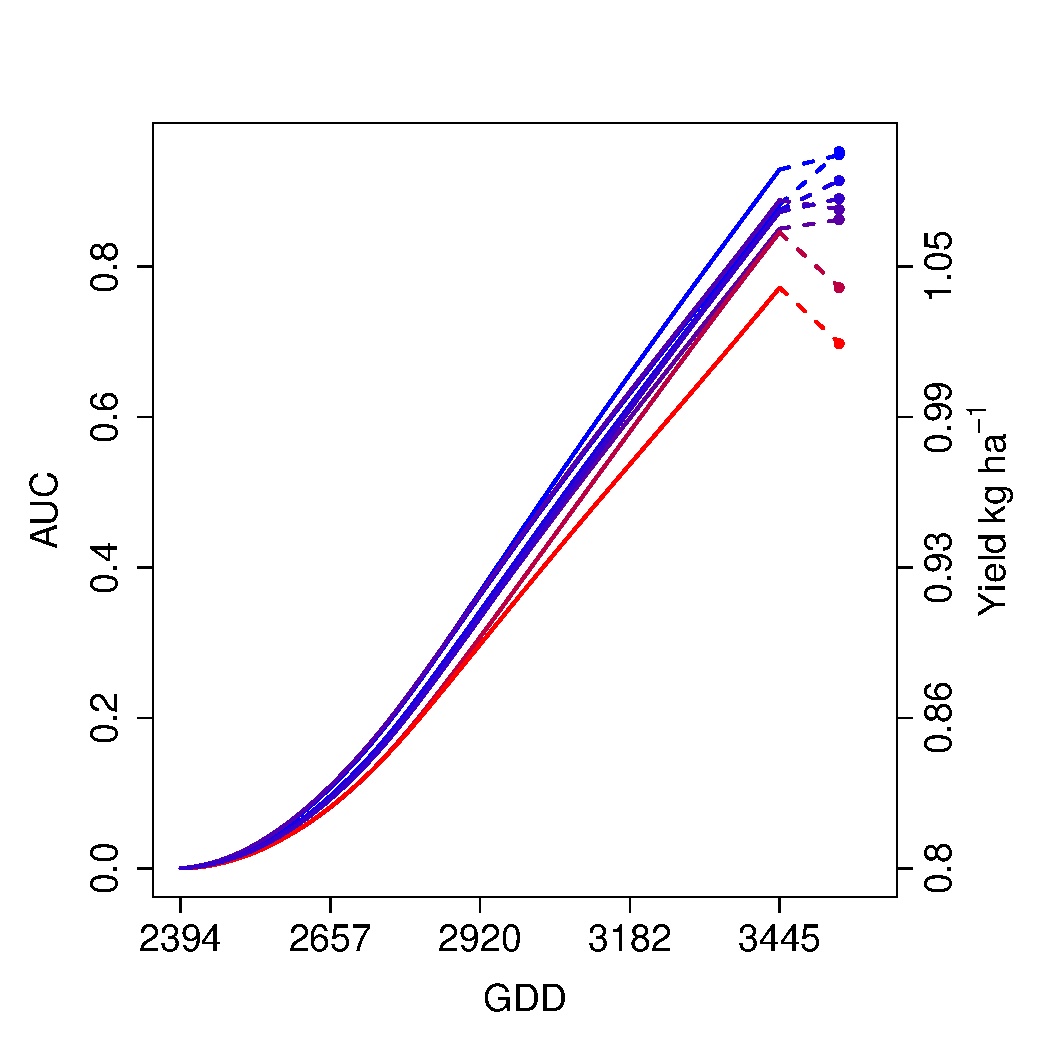
\includegraphics[width = 6cm]{AUC_ndvi_yld_h3_2019_geno8}};
  \end{scope}


  \begin{scope}[xshift=-6cm, yshift=-3cm, scale=0.3]
    \node () at (0,0) {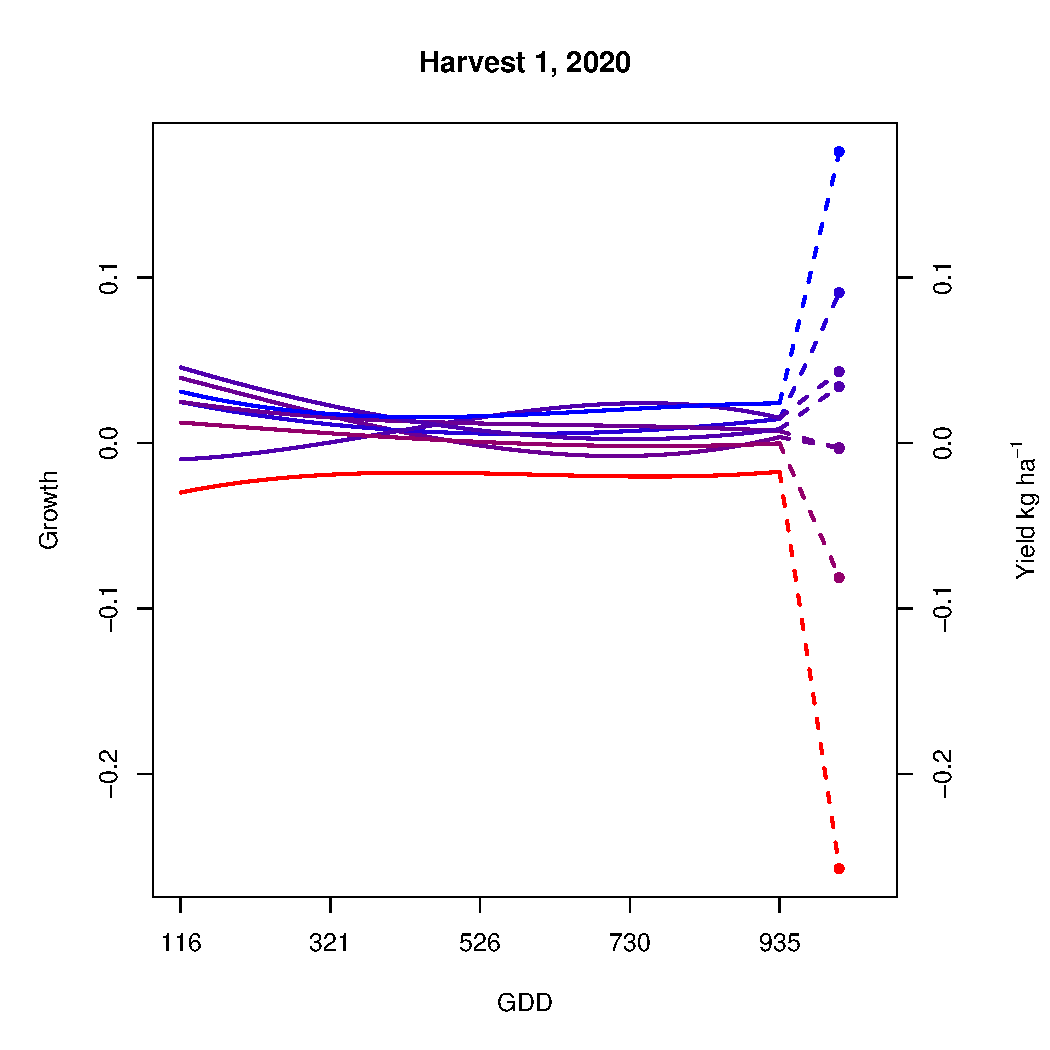
\includegraphics[width = 6cm]{growthCurveDeviations_ndvi_yld_h1_2020_geno8}};
  \end{scope}

  \begin{scope}[xshift=0cm, yshift=-3cm, scale=0.3]
    \node () at (0,0) {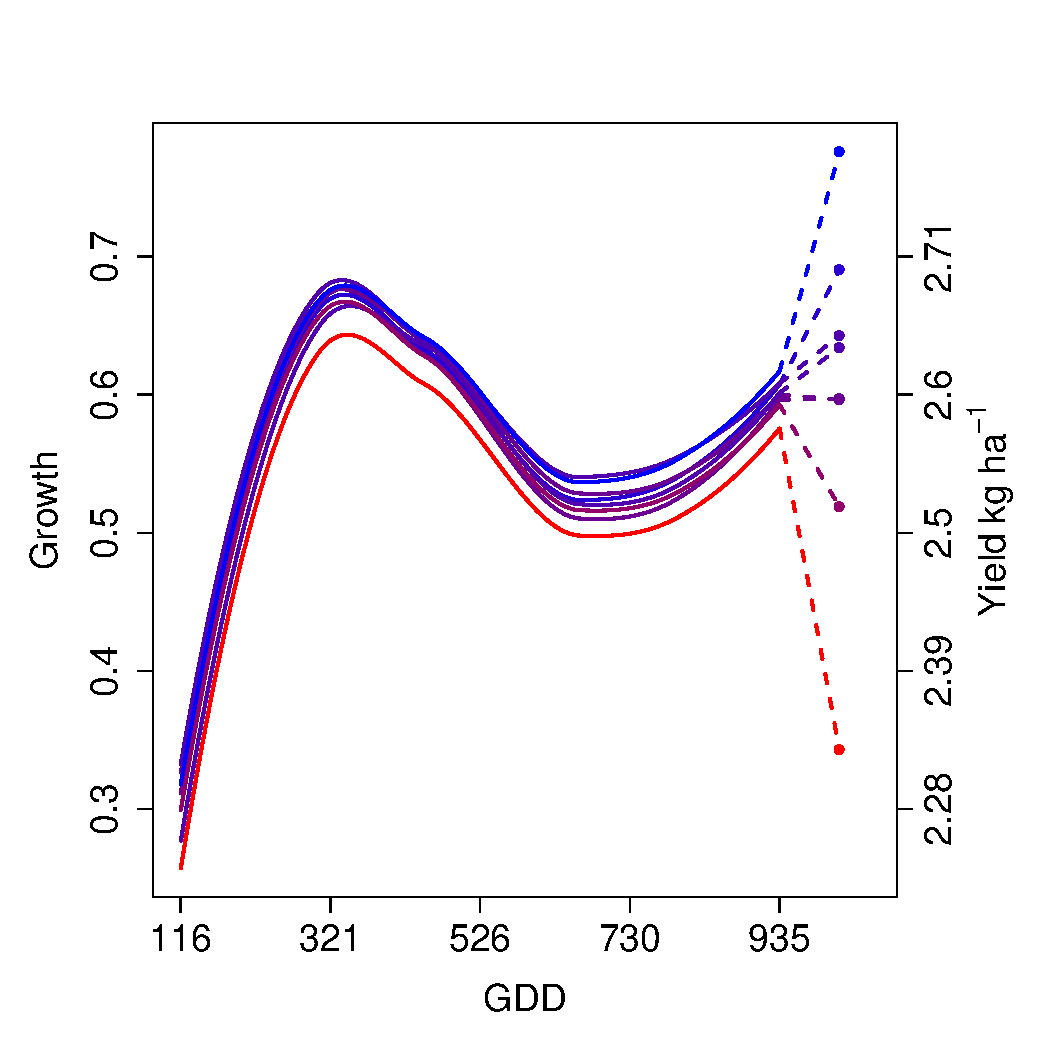
\includegraphics[width = 6cm]{growthCurvesWithMeanCurve_ndvi_yld_h1_2020_geno8}};
  \end{scope}

  \begin{scope}[xshift=6cm, yshift=-3cm, scale=0.3]
    \node () at (0,0) {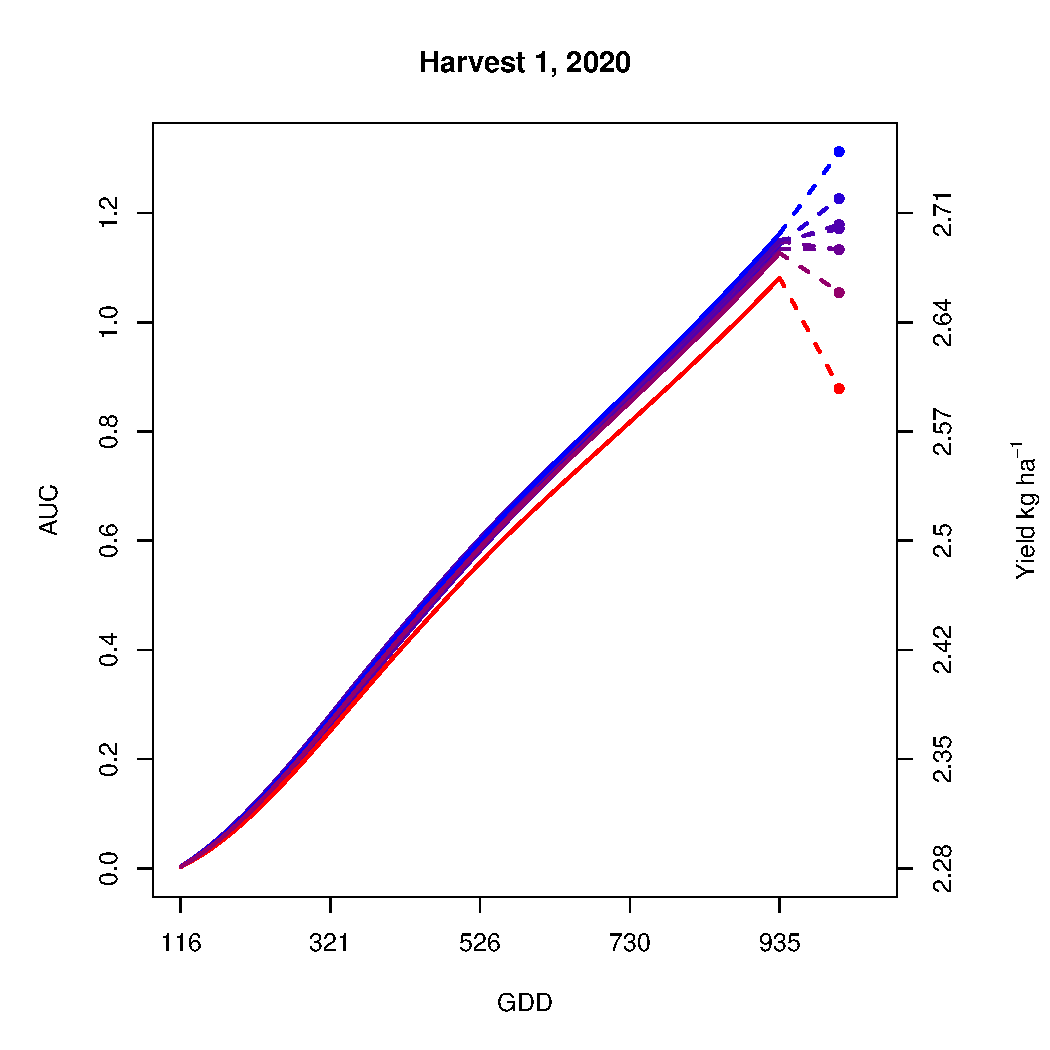
\includegraphics[width = 6cm]{AUC_ndvi_yld_h1_2020_geno8}};
  \end{scope}



  \begin{scope}[xshift=-6cm, yshift=-9cm, scale=0.3]
    \node () at (0,0) {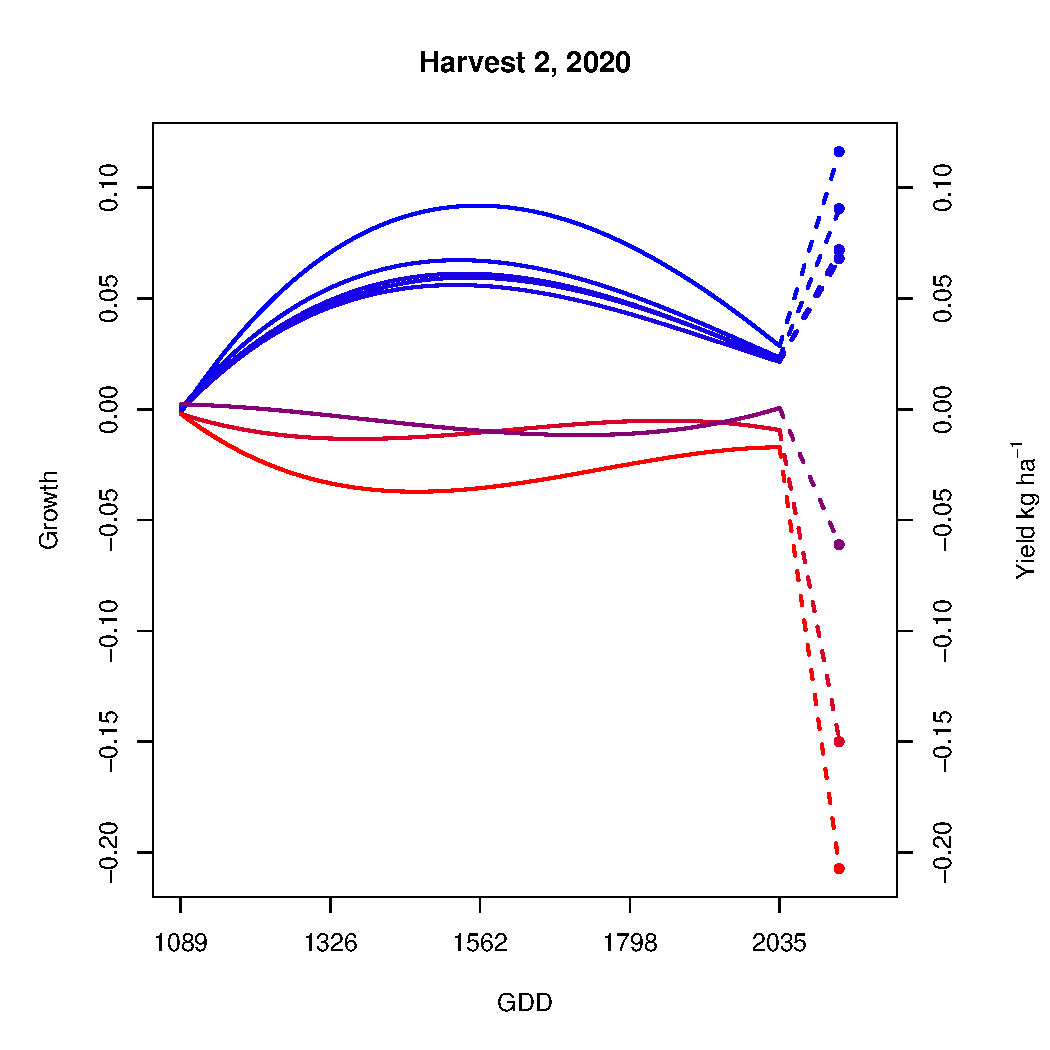
\includegraphics[width = 6cm]{growthCurveDeviations_ndvi_yld_h2_2020_geno8}};
  \end{scope}

  \begin{scope}[xshift=0cm, yshift=-9cm, scale=0.3]
    \node () at (0,0) {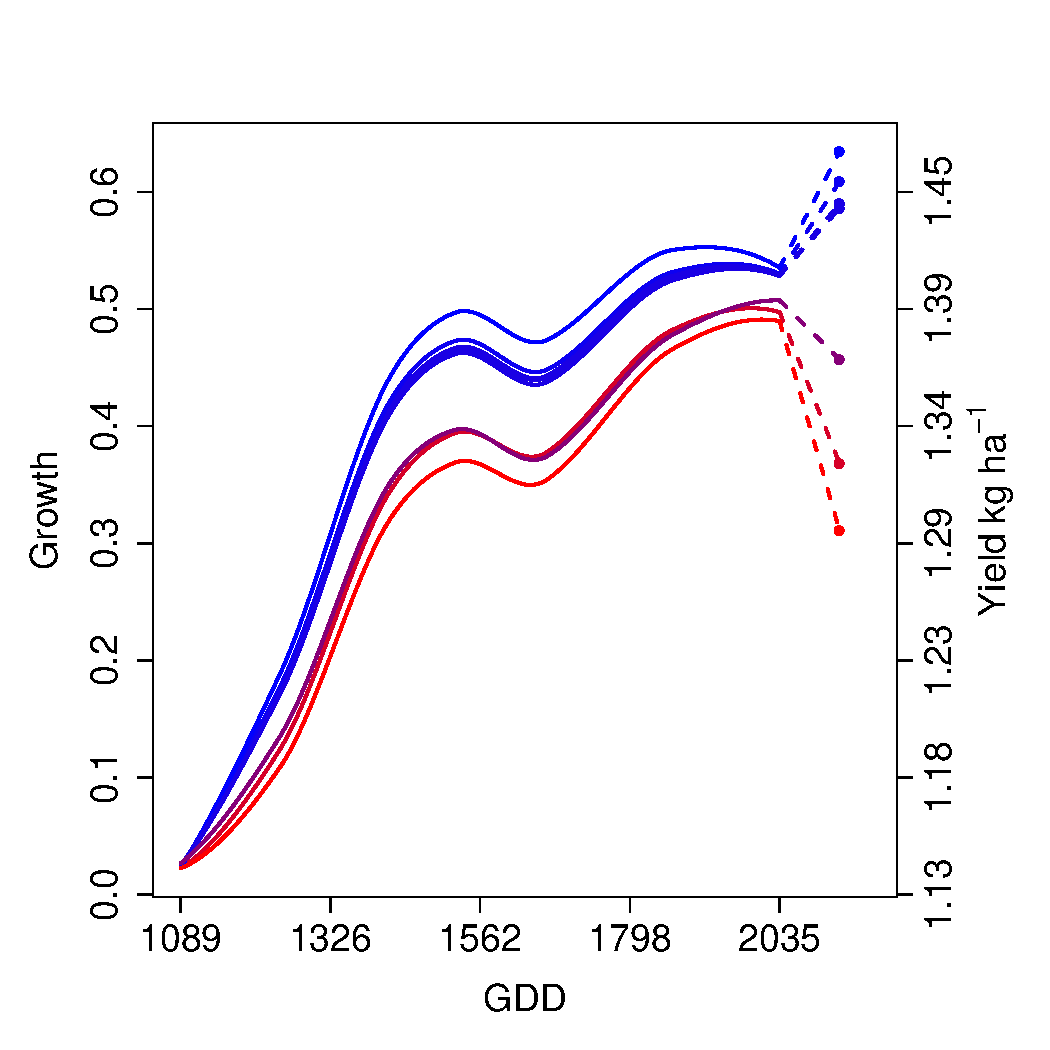
\includegraphics[width = 6cm]{growthCurvesWithMeanCurve_ndvi_yld_h2_2020_geno8}};
  \end{scope}

  \begin{scope}[xshift=6cm, yshift=-9cm, scale=0.3]
    \node () at (0,0) {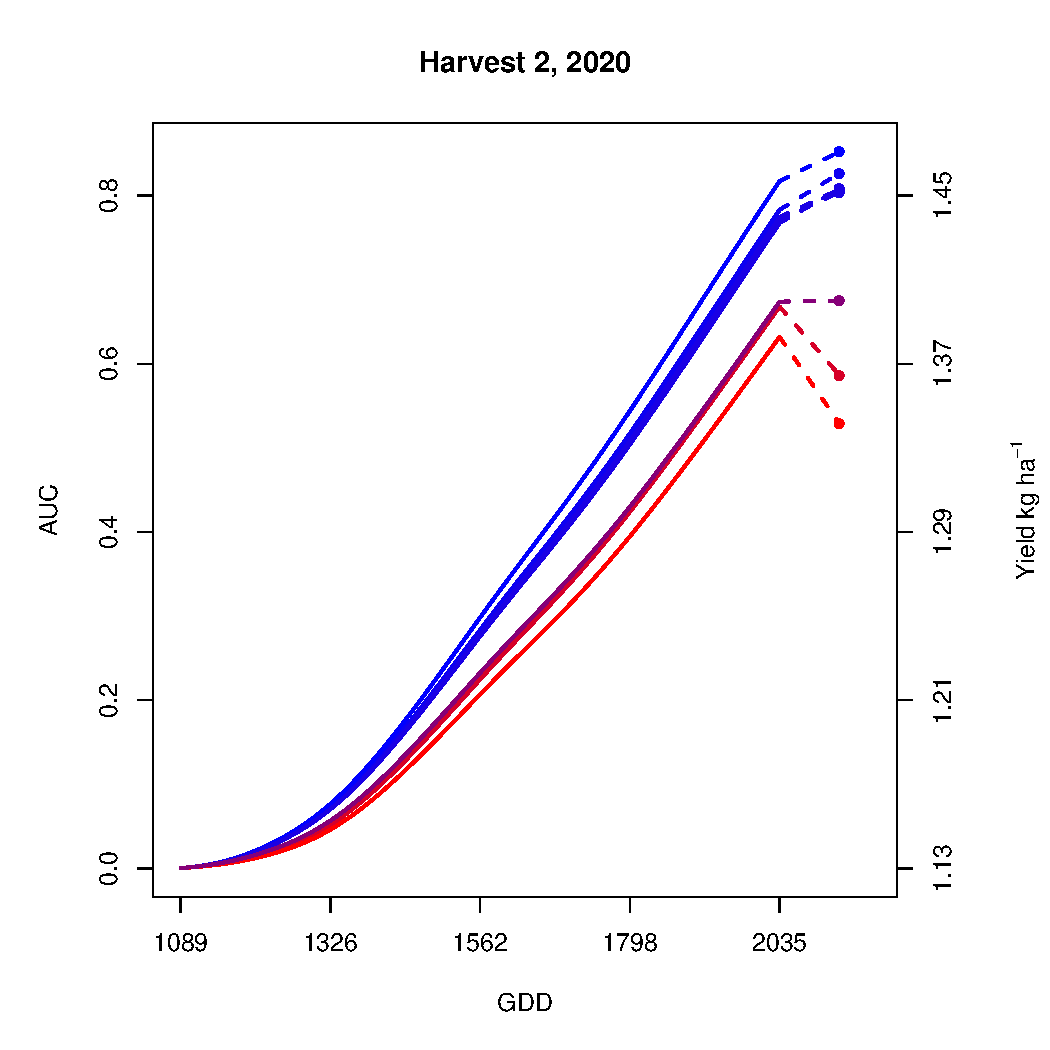
\includegraphics[width = 6cm]{AUC_ndvi_yld_h2_2020_geno8}};
  \end{scope}

 \end{tikzpicture}
\vspace{-1cm}
\caption{Genetic growth curve deviations, genetic growth curves with mean growth curve, and the area under the genetic growth curve for forage yield in four harvests. Blue = high FY, Red = low FY.}
\label{growthcurvesyld}
\end{figure}



\begin{figure}
\vspace{-2.3cm}
\hspace{-1cm}
 \begin{tikzpicture}

 \begin{scope}[xshift=-6cm, yshift=12cm, scale=0.3]
    \node () at (0,0) {\textbf{Growth curve deviations}};
  \end{scope}

\begin{scope}[xshift=0cm, yshift=12cm, scale=0.3]
    \node () at (0,0) {\textbf{Growth curves}};
  \end{scope}

\begin{scope}[xshift=6cm, yshift=12.2cm, scale=0.3]
    \node () at (0,0) {\begin{tabular}{c} \textbf{Area under the} \\ \textbf{growth curve (AUGC)} \end{tabular}};
  \end{scope}
%%%%%%%%%%%%%%%%%%
  \begin{scope}[xshift=-9cm, yshift=9cm, scale=0.3]
    \node[rotate = 90] () at (0,0) {CP Harvest 2, 2019};
  \end{scope}

\begin{scope}[xshift=-9cm, yshift=3cm, scale=0.3]
    \node[rotate = 90] () at (0,0) {NDF Harvest 3, 2019};
  \end{scope}

\begin{scope}[xshift=-9cm, yshift=-3cm, scale=0.3]
    \node[rotate = 90] () at (0,0) {CP Harvest 1, 2020};
  \end{scope}

\begin{scope}[xshift=-9cm, yshift=-9cm, scale=0.3]
    \node[rotate = 90] () at (0,0) {NDF Harvest 2, 2020};
  \end{scope}

%%%%%%%%%%%

  \begin{scope}[xshift=-6cm, yshift=9cm, scale=0.3]
    \node () at (0,0) {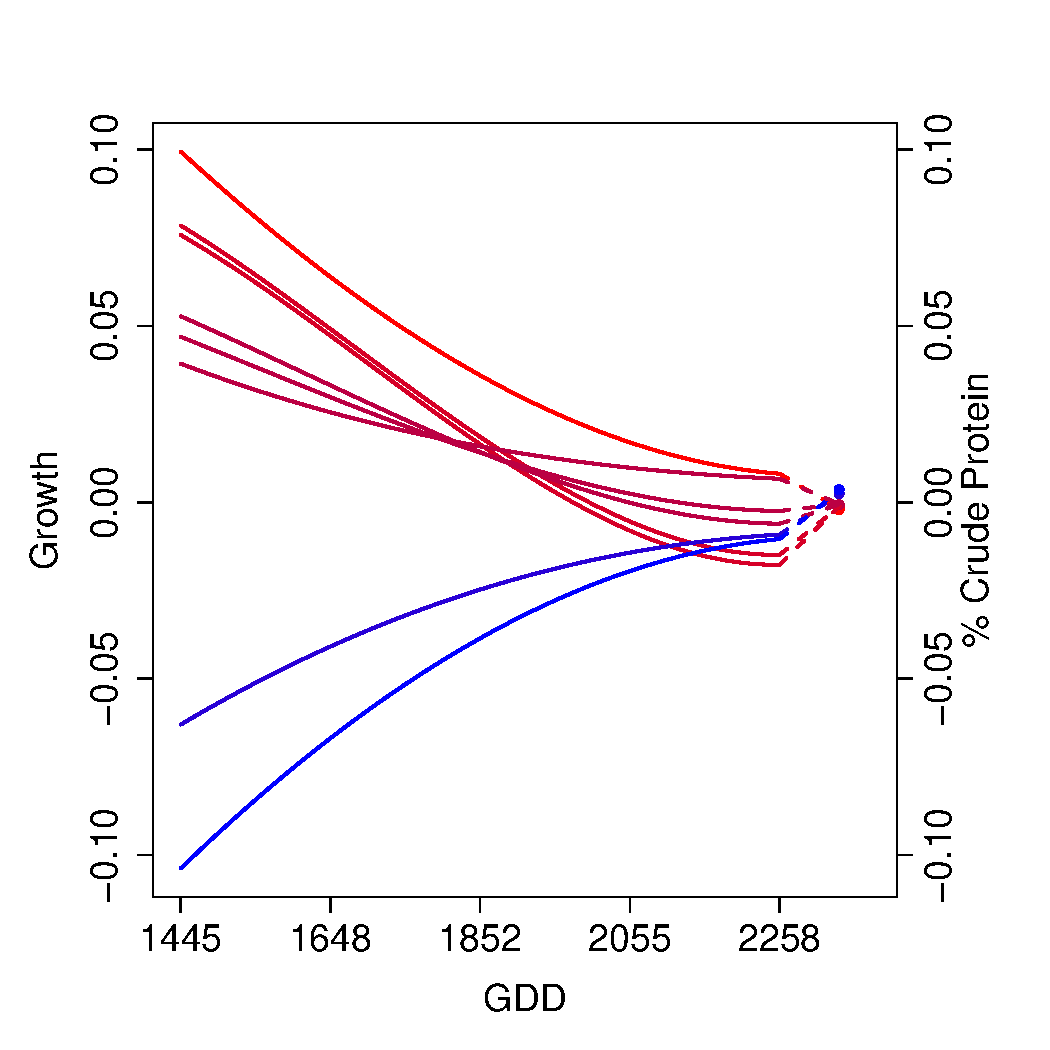
\includegraphics[width = 6cm]{growthCurveDeviations_ndvi_CP_h2_2019_geno8}};
  \end{scope}

  \begin{scope}[xshift=0cm, yshift=9cm, scale=0.3]
    \node () at (0,0) {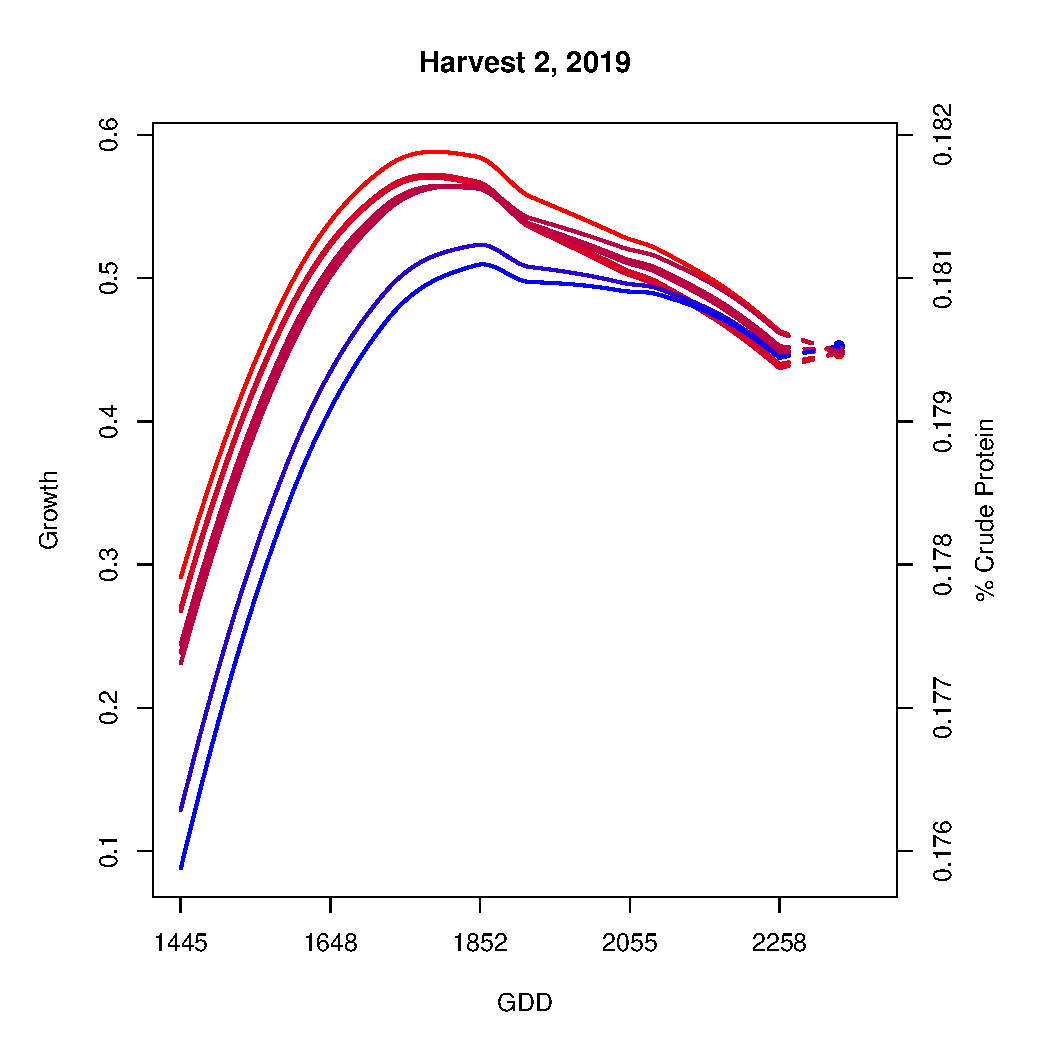
\includegraphics[width = 6cm]{growthCurvesWithMeanCurve_ndvi_CP_h2_2019_geno8}};
  \end{scope}

  \begin{scope}[xshift=6cm, yshift=9cm, scale=0.3]
    \node () at (0,0) {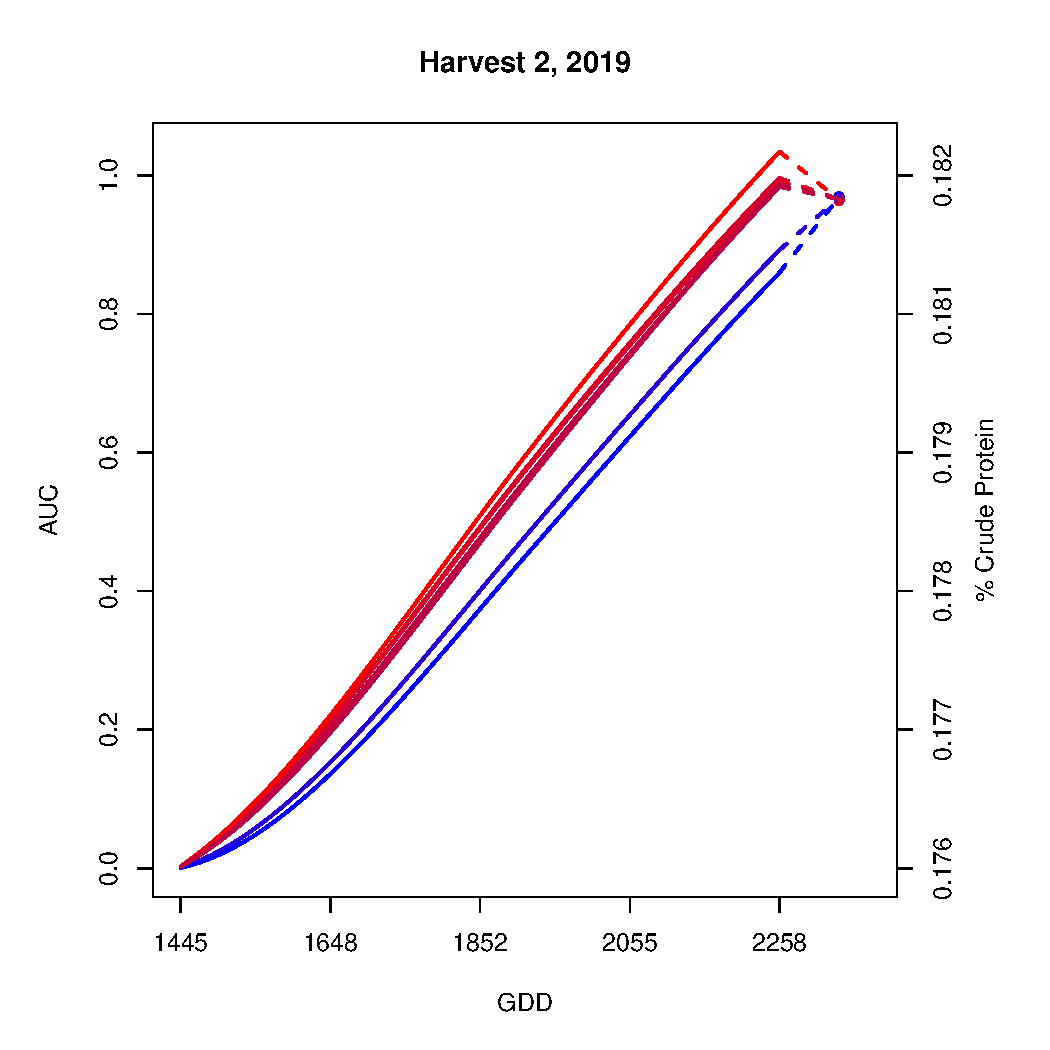
\includegraphics[width = 6cm]{AUC_ndvi_CP_h2_2019_geno8}};
  \end{scope}


  \begin{scope}[xshift=-6cm, yshift=3cm, scale=0.3]
    \node () at (0,0) {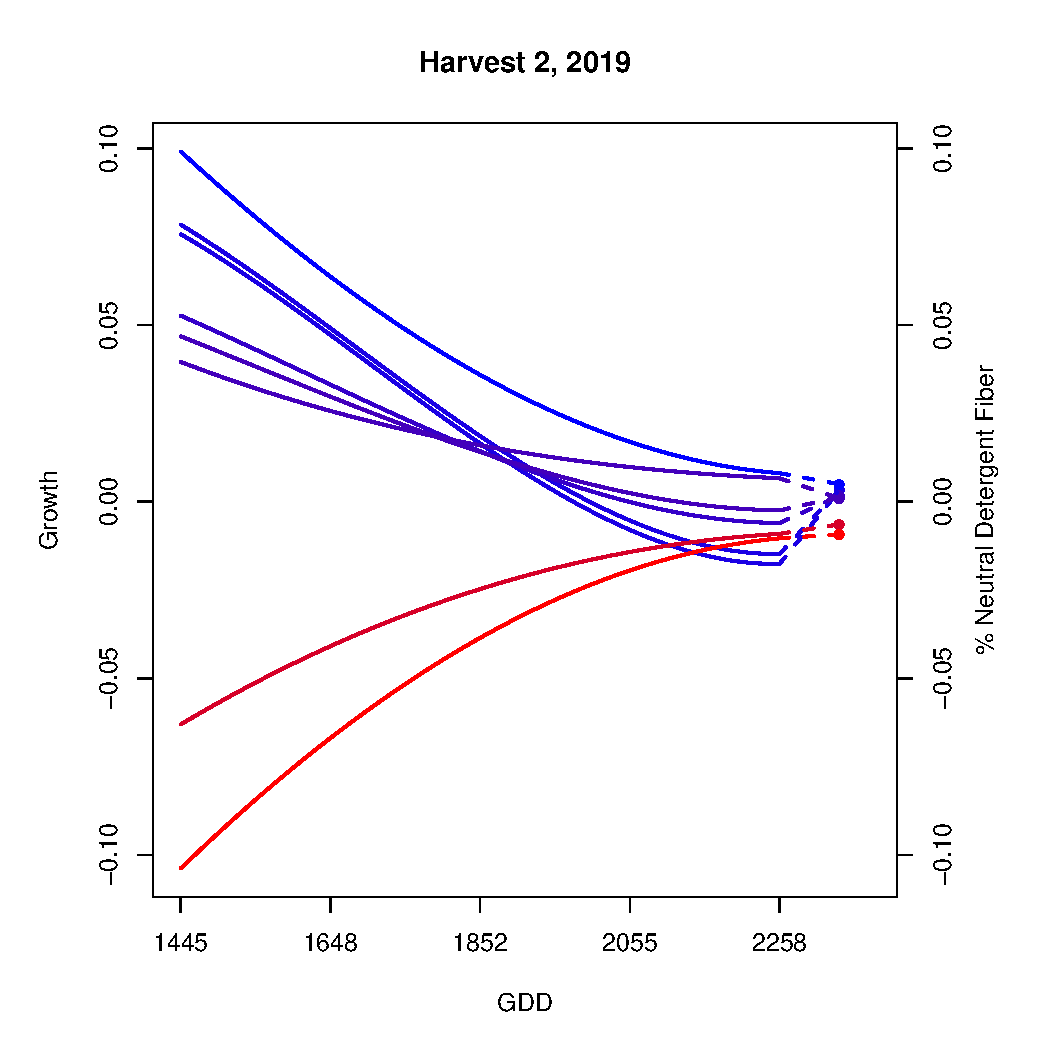
\includegraphics[width = 6cm]{growthCurveDeviations_ndvi_NDF_h2_2019_geno8}};
  \end{scope}

  \begin{scope}[xshift=0cm, yshift=3cm, scale=0.3]
    \node () at (0,0) {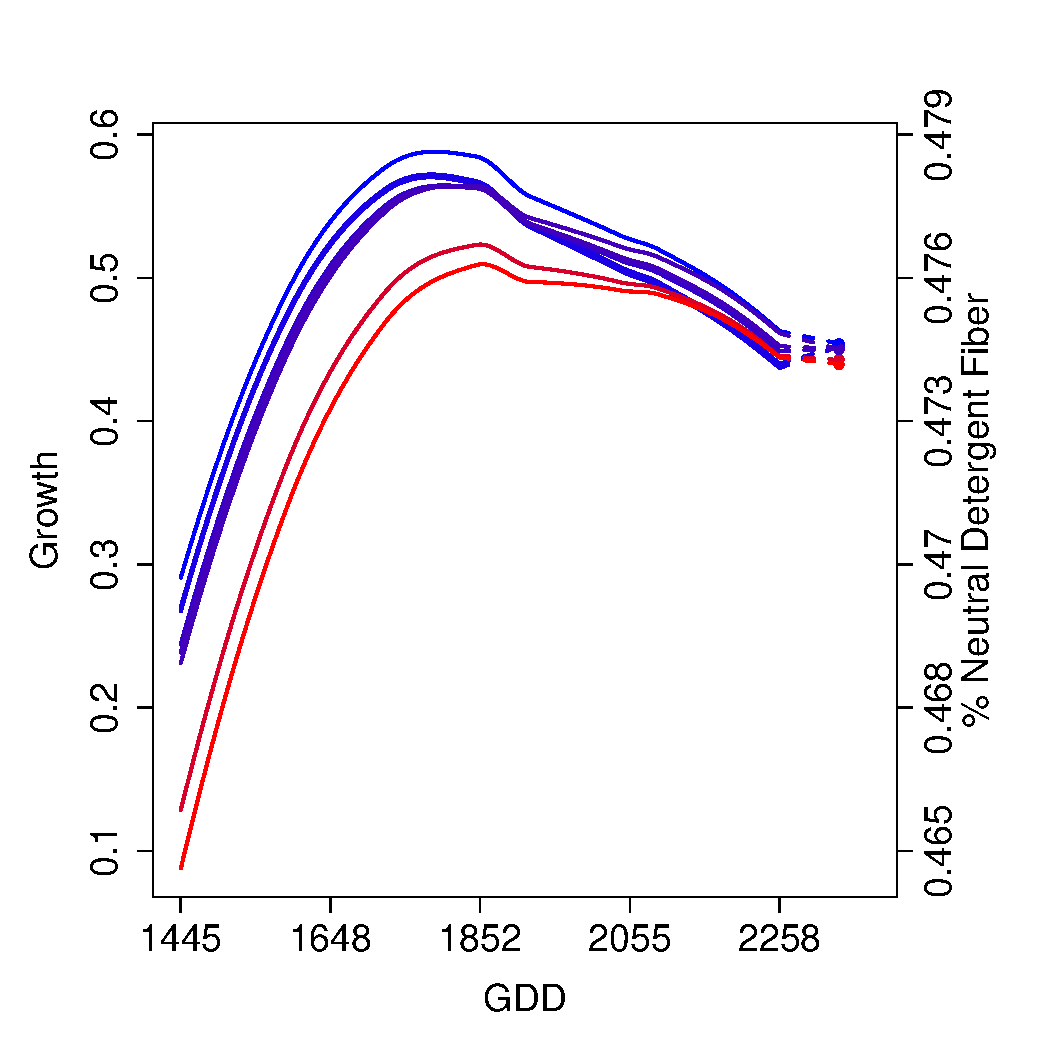
\includegraphics[width = 6cm]{growthCurvesWithMeanCurve_ndvi_NDF_h2_2019_geno8}};
  \end{scope}

  \begin{scope}[xshift=6cm, yshift=3cm, scale=0.3]
    \node () at (0,0) {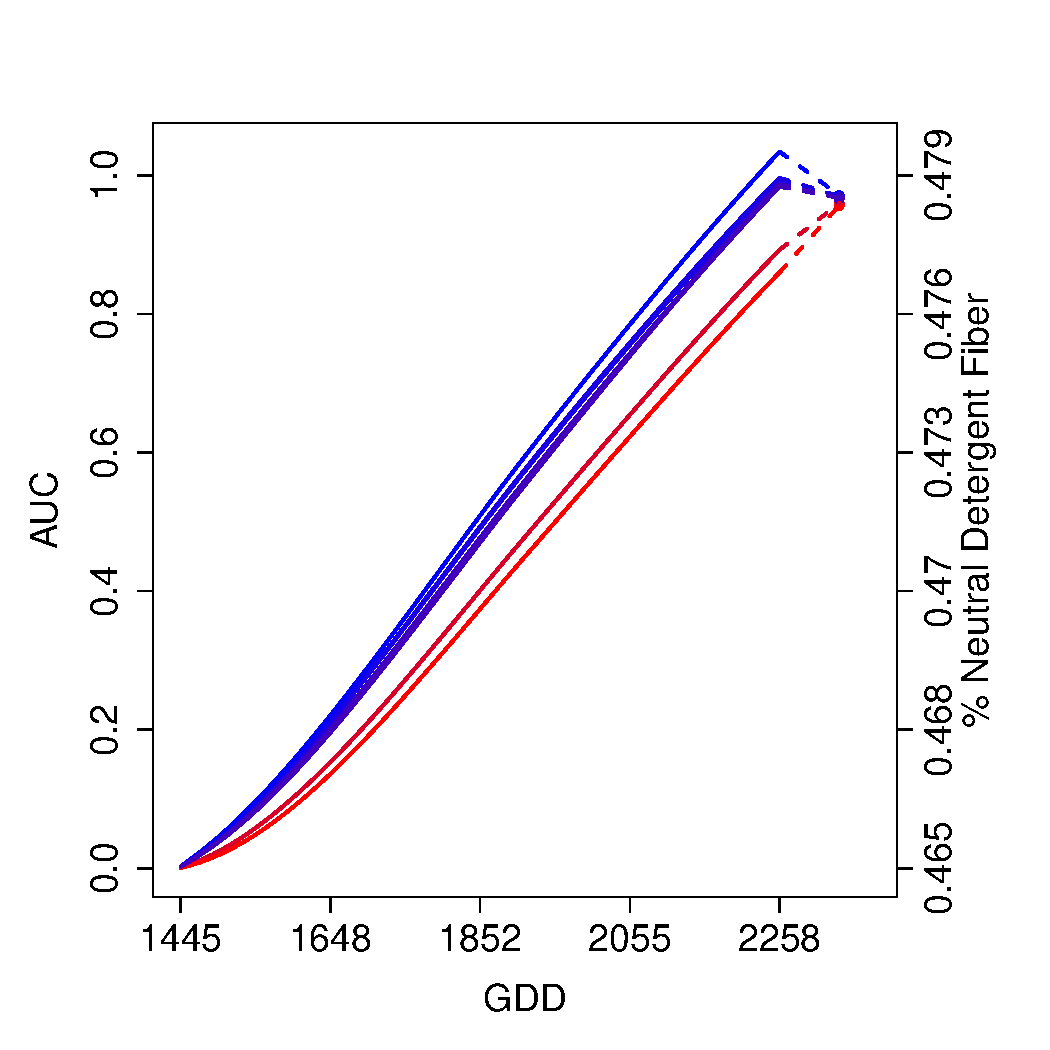
\includegraphics[width = 6cm]{AUC_ndvi_NDF_h2_2019_geno8}};
  \end{scope}


  \begin{scope}[xshift=-6cm, yshift=-3cm, scale=0.3]
    \node () at (0,0) {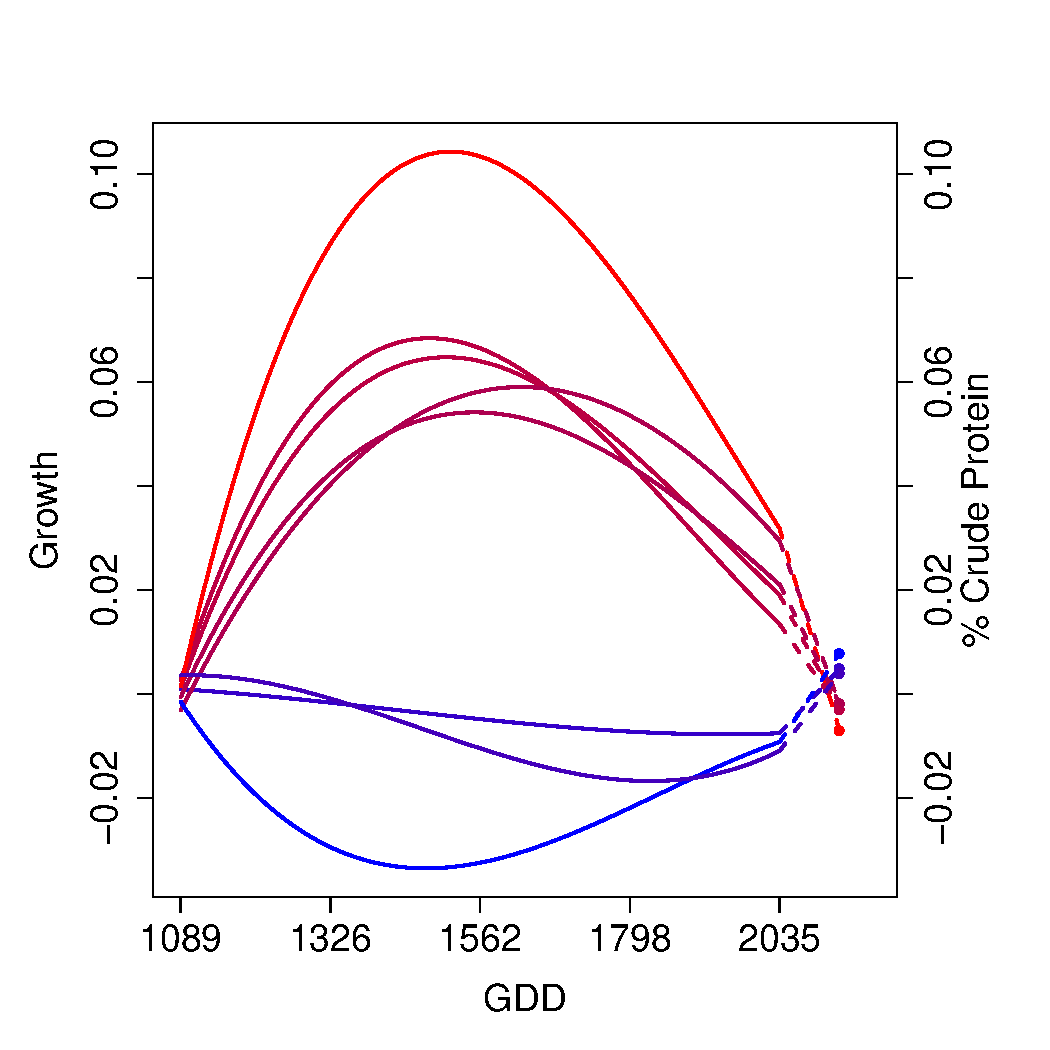
\includegraphics[width = 6cm]{growthCurveDeviations_ndvi_CP_h2_2020_geno8}};
  \end{scope}

  \begin{scope}[xshift=0cm, yshift=-3cm, scale=0.3]
    \node () at (0,0) {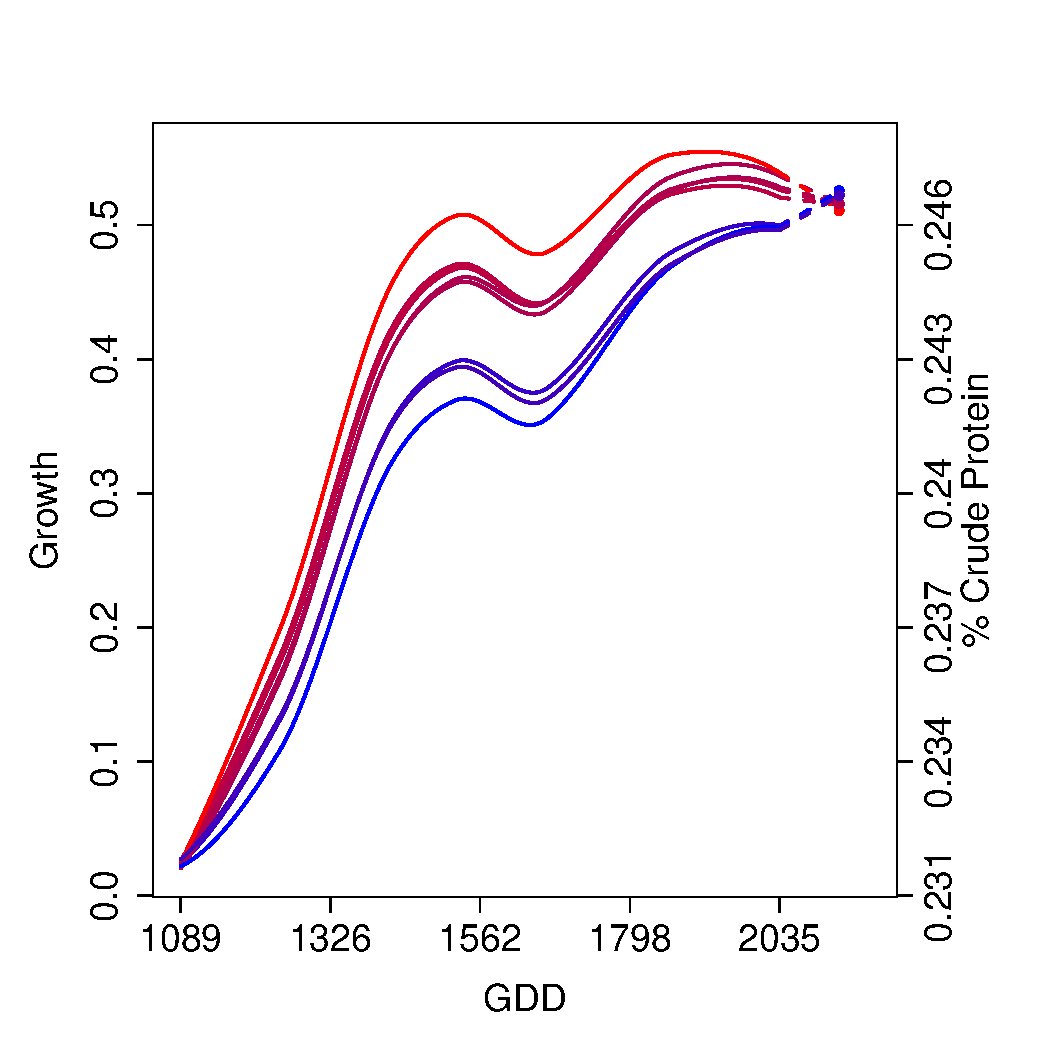
\includegraphics[width = 6cm]{growthCurvesWithMeanCurve_ndvi_CP_h2_2020_geno8}};
  \end{scope}

  \begin{scope}[xshift=6cm, yshift=-3cm, scale=0.3]
    \node () at (0,0) {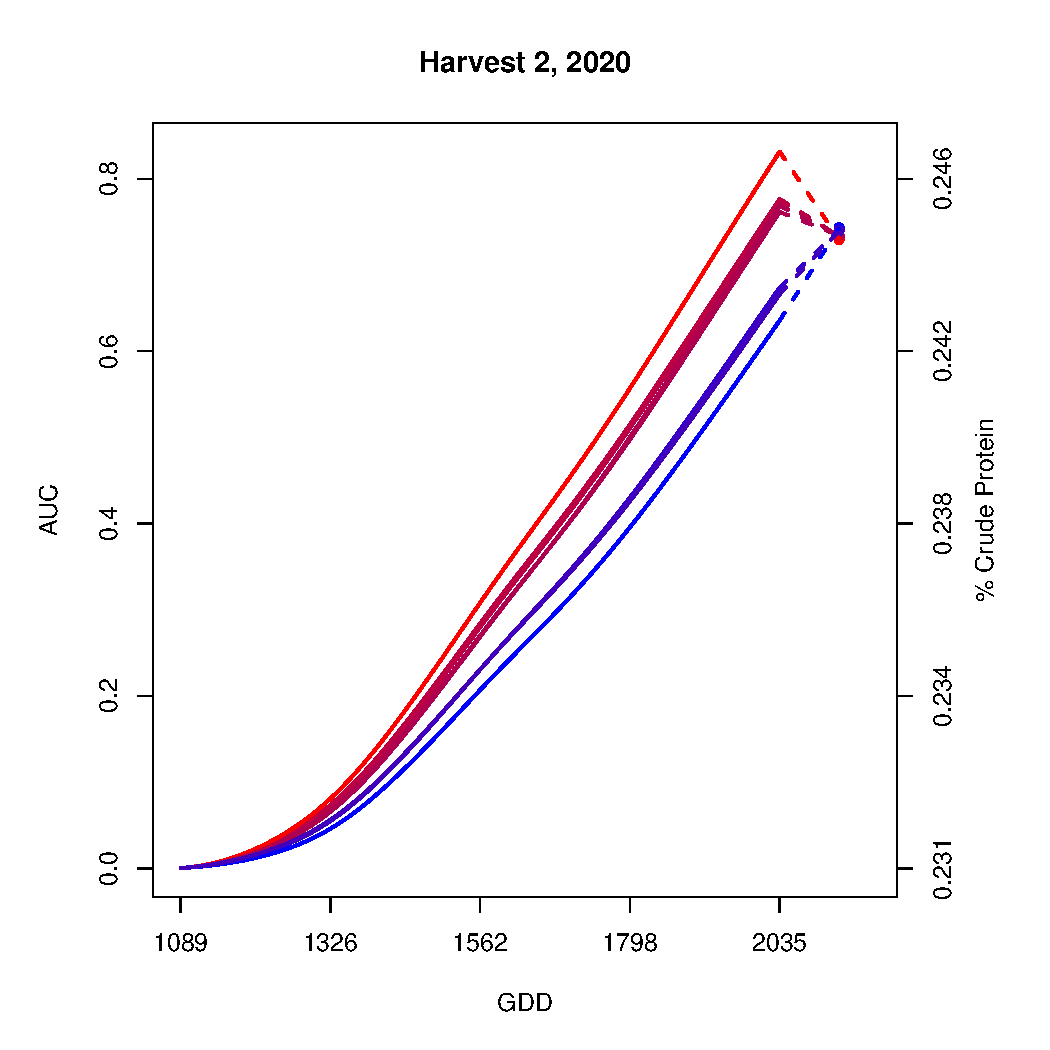
\includegraphics[width = 6cm]{AUC_ndvi_CP_h2_2020_geno8}};
  \end{scope}



  \begin{scope}[xshift=-6cm, yshift=-9cm, scale=0.3]
    \node () at (0,0) {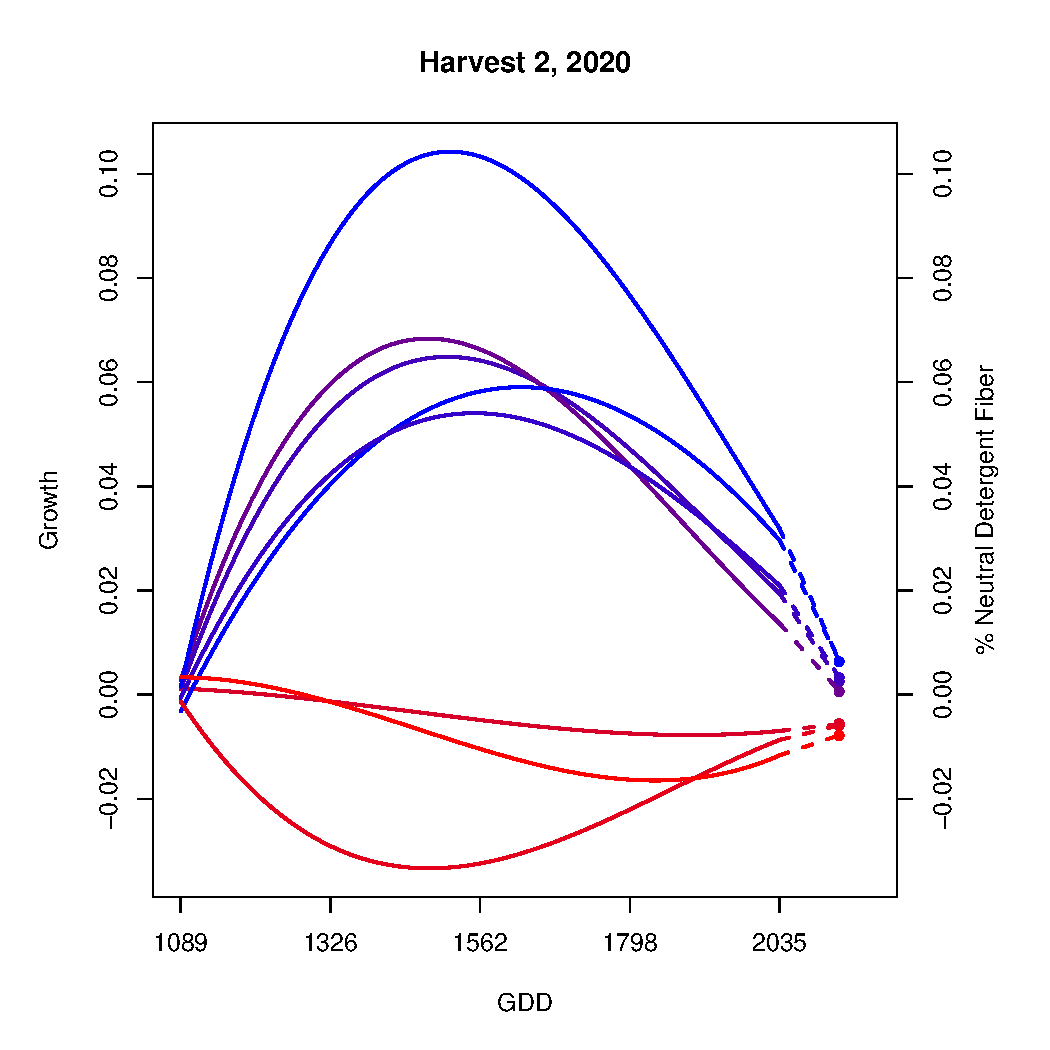
\includegraphics[width = 6cm]{growthCurveDeviations_ndvi_NDF_h2_2020_geno8}};
  \end{scope}

  \begin{scope}[xshift=0cm, yshift=-9cm, scale=0.3]
    \node () at (0,0) {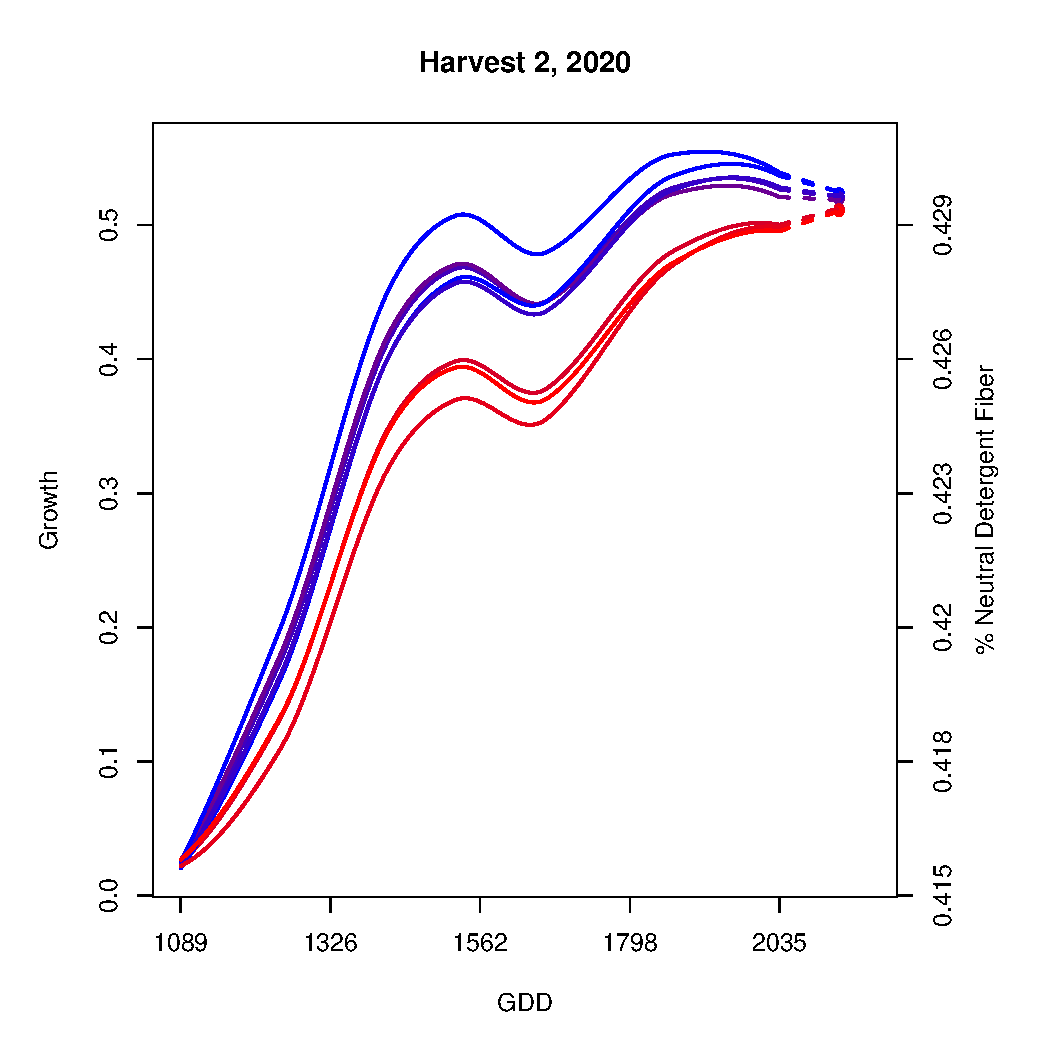
\includegraphics[width = 6cm]{growthCurvesWithMeanCurve_ndvi_NDF_h2_2020_geno8}};
  \end{scope}

  \begin{scope}[xshift=6cm, yshift=-9cm, scale=0.3]
    \node () at (0,0) {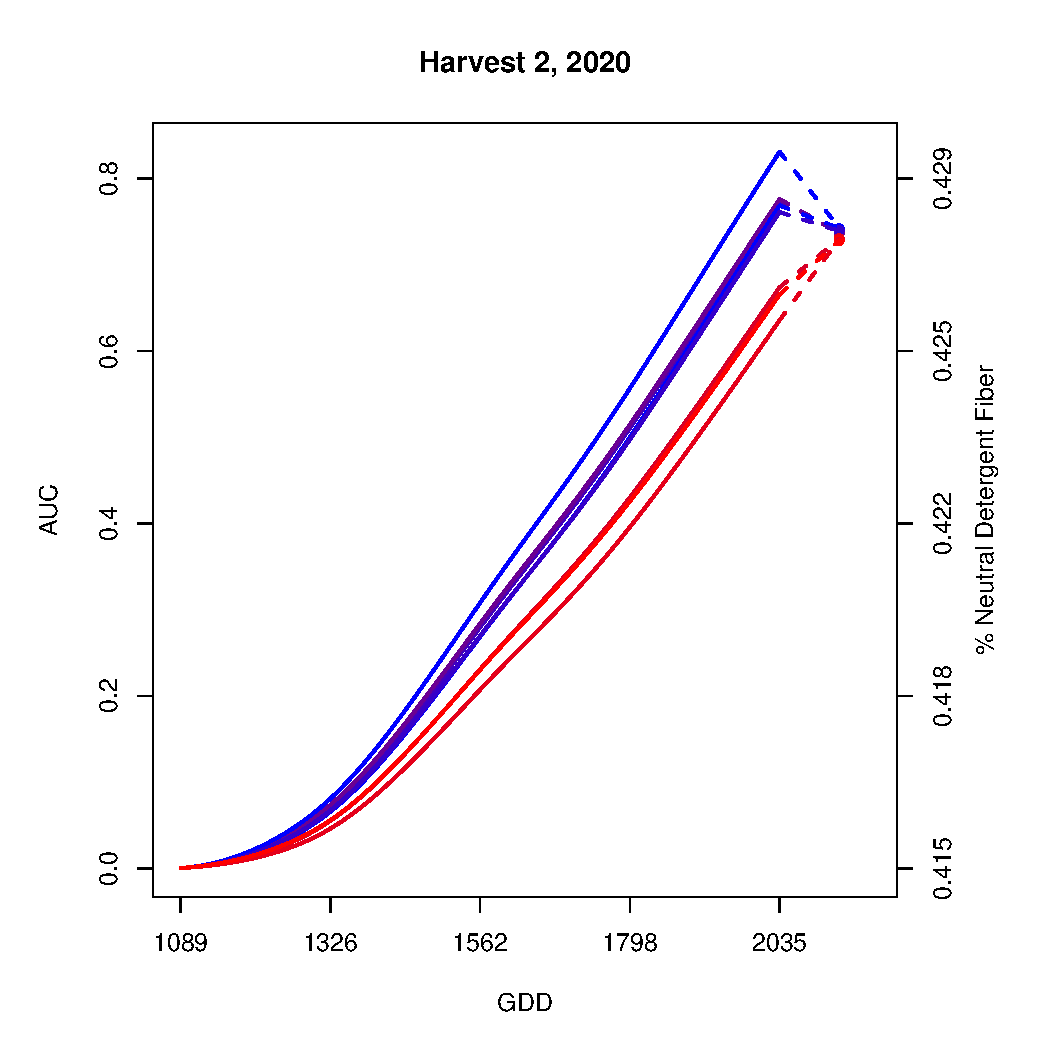
\includegraphics[width = 6cm]{AUC_ndvi_NDF_h2_2020_geno8}};
  \end{scope}

 \end{tikzpicture}
\vspace{-1cm}
\caption{Genetic growth curve deviations, genetic growth curves with mean growth curve, and the area under the genetic growth curve for CP and NDF in two harvests. Blue = high CP or NDF, Red = low CP or NDF.}
\label{growthcurvesqual}
\end{figure}

Shapes in growth curves differed for each harvest, but some trends were evident (Figure \ref{growthcurvesyld}). In particular, populations with faster regrowth tended to have higher yields than those with slower regrowth, an observation that has no doubt not escaped forage breeders since the profession has existed. The effect was less evident in harvest 1, 2020, the only harvest we sampled after winter dormancy, but it is unclear if regrowth after winter is less important, or if this was a unique event. Quality measures tended to follow their genetic correlations with forage yield (see Table, with high protein (CP) associated with lower yields and high digestible carbohydrates (NDF) associated with high yields, despite the lack of much genetic variability for CP in 2019 and NDF in 2020 (Figure \ref{growthcurvesqual}). 

The $L0$ Legendre parameter coefficient, akin to an intercept, or ``mean'' genetic value  was consistently highly correlated with Forage Yield, while the linear ($L1$), quadratic ($L2$) and and cubic ($L3$) Legendre polynomial components were more variable. Higher order Legendre polynomial coefficients also tended to be highly positively or negatively correlated with one another, but these trends changed from harvest to harvest. 

The area under the growth curve (AUGC) corresponded well with final forage biomass, suggesting these growth curves can be used to estimate total photosynthate partitioning to the harvested product, which in this case is above ground biomass. Mean growth curves are subject to environmental effects, such as temperature and precipitation. The change in genetic growth curve deviations from harvest to harvest suggests that varieties respond differentially under different environmental stresses. Further investigation is needed to determine if these environmental conditions had an effect on the  mean as well as the gene.

% should plot precip with growth curve to show that drought stress reduces growth!


In general, the number of populations under evaluation in this study was small, and a better understanding of how growth curves are related forage production would need more populations, and be evaluated from stand establishment through at least the third year. It is unclear from this study what effect stand persistence has on these growth parameters, but should be a target of future research. 


% - Growth curves and relationships between curve and forage yield

% - Area under the curve and relationship to forage yields, quality

\section{Conclusion}

% - Other linear and non-linear indices should be investigated
% - larger sample sizes needed to validate and decipher more consistent trends
% - inclusion of genetic covariance important for prediction, perhaps more than VIs?

We find that estimating genetic relationships between populations is a valid approach that can be used for genomic prediction and selection, while drastically increasing predictability of unobserved traits. High throughput phenotypes such as vegetative indices taken with a multi-spectral camera equipped UAV have the potential to help reduce the phenotyping necessary to get good estimates of population performance. There appears to be significant genetic variability for growth and development that is associated with forage yield and quality, even in this small study. What is unclear from this study is to what degree these curves and end use traits are influenced by dormancy ratings and maturity, and whether these relationships can be changed. Clearly, the ideal variety will yield well, regrow quickly, have high protein and high digestible carbohydrates while maintaining good stand persistence. As we observe more populations in more environments, monitoring trials with UAVs has the potential to start to dissect these relationships as the picture of \emph{how} the genetics of growth and development leads to better end-use traits. An important question will be how plasticity in growth curves leads to yield and quality stability across varying environmental stressors such as heat and drought. 

This research has in part been used as preliminary evidence for submission of a grant proposal to FFAR Seeding Solutions: with a combined budget of \$767,605, and will include a larger three year study of 24 alfalfa varieties evaluated at Cornell, and 24 varieties evaluated for two years at New Mexico State University. The effects growth and development of other crops, including wheat at Virginia Tech and other grain, fiber and oil crops from BASF and Lima Grain will be investigated along with alfalfa in this FFAR project, pending a positive funding decision. 

\clearpage

\section{Acknowledgments}

We want to express special appreciation to the Noble Research Institute for providing the alfalfa genome assembly, without which this work would not have been possible. In particular to we would like to recognize Michael Udvardi and Maria Monteros for providing the data, Andrew Segna for working to establish an MTA and to Andrew Farmer, who was integral to the graciously worked through several early alignment questions with us.  We are grateful to Don Viands and Julie Hansen and the rest of the  the Forage Breeding and genetic program team at Cornell university, for allowing us to image and genotype their materials. We hope that the collaboration formed for this project is sustained well into the future of the forage breeding program at Cornell University. % Finally, we wish Professor Donald Viands a happy and restful retirement. 


\printbibliography

% \section{References}
% Segovia-Lerma, A., Murray, L. W., Townsend, M. S., and I. M. Ray. 2004. \emph{Population-based diallel analyses among nine historically recognized alfalfa germplasms}. Theor. Appl. Genet., 109(8), 1568-1575.\\

% Weir, B.S. and W.G. Hill. 2002. \emph{Estimating F-Statistics}. Annu. Rev. Genet. 2002. 36:721–50. doi: 10.1146/annurev.genet.36 050802.093940

\end{document}
